\documentclass[aspectratio=169,10pt]{beamer}
\graphicspath{{figures/}} % Setting the graphicspath

% Theme settings
\usetheme{Madrid}
\usecolortheme{default}
\setbeamertemplate{navigation symbols}{}   % removes navigation symbols such as 'next page'
\setbeamertemplate{footline}{}             % remove line with name, date, page nr. 
\setbeamercolor*{frametitle}{bg=white}     % remove background from frametitle
\usepackage{caption}
\captionsetup[figure]{labelformat=empty}% redefines the caption setup of the figures environment in the beamer class.
\setbeamersize{text margin left=20pt,text margin right=10pt}

\usefonttheme[onlymath]{serif}

\definecolor{Red}{rgb}{1,0,0}
\definecolor{Green}{rgb}{0,1,0}
\definecolor{Blue}{rgb}{0,0,1}
\definecolor{Gray}{gray}{0.9}
\definecolor{springgreen}   {cmyk}{0.26, 0   , 0.76, 0   }
\definecolor{olivegreen}    {cmyk}{0.64, 0   , 0.95, 0.40}
\definecolor{emerald}       {cmyk}{1   , 0   , 0.50, 0   }
\definecolor{junglegreen}   {cmyk}{0.99, 0   , 0.52, 0   }
\definecolor{seagreen}      {cmyk}{0.69, 0   , 0.50, 0   }
\definecolor{green}         {cmyk}{1   , 0   , 1   , 0   }
\definecolor{forestgreen}   {cmyk}{0.91, 0   , 0.88, 0.12}
\definecolor{pinegreen}     {cmyk}{0.92, 0   , 0.59, 0.25}
\definecolor{sepia}         {cmyk}{0   , 0.83, 1   , 0.70}
\definecolor{cerulean}      {cmyk}{0.94, 0.11, 0   , 0   }
\definecolor{salmon}        {cmyk}{0   , 0.53, 0.38, 0   }
\definecolor{greenyellow}   {cmyk}{0.15, 0   , 0.69, 0   }
\definecolor{arsenic}       {rgb}{0.23, 0.27, 0.29}
\definecolor{britishracinggreen}{rgb}{0.0, 0.26, 0.15}
\definecolor{oxfordblue}{rgb}{0.0, 0.13, 0.28}
\definecolor{bostonuniversityred}{rgb}{0.8, 0.0, 0.0}
\definecolor{goldenyellow}{rgb}{1.0, 0.87, 0.0}

\definecolor{darkgreen}{rgb}{0.0, 0.5, 0.13}
\definecolor{darkred}{rgb}{0.55, 0.0, 0.0}

\newcommand{\arrowdownunder}{\begin{center}$\big\downarrow$\end{center}\vspace{-0.3cm}}
\newcommand{\mycolutitle}[1]{\vspace{-0.7cm}\begin{center}#1\end{center}\vspace{-0.1cm}}

\newcommand\ballref[1]{%
\tikz \node[circle, shade,ball color=structure.fg,inner sep=0pt,%
  text width=8pt,font=\tiny,align=center] {\color{white}\ref{#1}};
}

%\fontsize{4pt}{5}\selectfont

%======================= import packages =======================
\usepackage{pifont}       % Pi fonts (Digbats, symbol, etc.)
\usepackage{graphicx}     % More options for \includegraphics
\usepackage{tikz}
\usepackage{appendixnumberbeamer} % separate appendix numbering
\usepackage{booktabs}
\usepackage{hyperref}
\usepackage{tabularx}



%======================= tikz settings =======================
\usetikzlibrary{shapes, arrows}
\usetikzlibrary{decorations.pathreplacing}
\usetikzlibrary{positioning, calc}
\tikzstyle{fitted} = [rectangle, minimum width=5cm, minimum height=1cm, text centered, draw=black, fill=red!30]
\tikzstyle{operations} = [rectangle, rounded corners, minimum width=2cm,text centered, draw=black, fill=red!30]
\tikzstyle{roundtext} = [rectangle, rounded corners, minimum width=2cm, minimum height=0.8cm, text centered, draw=black, fill=red!30]
\tikzstyle{n3py} = [rectangle, rounded corners, minimum width=3cm, minimum height=1cm, text centered, draw=black, fill=green!30]
\tikzstyle{myarrow} = [thick,->,>=stealth]
\tikzstyle{line} =[draw, -latex']
\tikzstyle{decision} = [diamond, draw, fill=red!20, text width=7.5em, text centered,  inner sep=0pt, minimum height=2em, aspect=4]
\tikzstyle{cloud} = [draw, ellipse,fill=green!20, minimum height=2em]
\tikzstyle{inout} = [rectangle, draw, fill=green!20, text width=9.5em, text centered, rounded corners, minimum height=2em, minimum width=10em]
\tikzstyle{block}=[rectangle, draw, fill=blue!20, text width=9.5em, 
                   text centered, rounded corners, minimum height=2em, 
                   minimum width=10em]
\tikzstyle{arrow} = [thick,->,>=stealth]

\pgfdeclarelayer{bg}    % declare background layer
\pgfsetlayers{bg,main}  % set the order of the layers (main is the standard layer)

%======================= page numbering =======================
\addtobeamertemplate{navigation symbols}{}{ \usebeamerfont{footline}
  \insertframenumber / \inserttotalframenumber \hspace*{2mm} \\ \vspace*{1mm} 
}


%=================================== colors ===================================
\definecolor{RoyBlue}{RGB}{22, 46, 69}
\definecolor{RoyGrey}{RGB}{64, 88, 128} 

\newcommand{\hlme}[1]{{\color{red}\bf #1}} % highlihgt me

\setbeamercolor{structure}{fg=RoyBlue} % itemize, enumerate, etc
\setbeamercolor{frametitle}{fg=RoyGrey}
 \setbeamercolor{section in head/foot}{bg=RoyBlue}


%======================= add progress dots to headline =======================
\setbeamertemplate{headline}{%
    \begin{beamercolorbox}[ht=4mm,dp=4mm]{section in head/foot}
        \insertnavigation{\paperwidth}
    \end{beamercolorbox}%
}%
\makeatother


%======================= add section title page =======================
\AtBeginSection[]{
  \begin{frame}
  \vfill
  \centering
    \usebeamerfont{title}\insertsectionhead\par%
  \vfill
  \end{frame}
}


%=================================== titlepage ===================================
\title{NNPDF4.0: Towards a new generation of PDFs using ML}
\date{ML4Jets 2021, 6 July 2021}
\author{Roy Stegeman}
\institute{University of Milan and INFN Milan}
\titlegraphic{\vspace*{6mm}
    
\includegraphics[height=0.8cm]{logos/LOGO-ERC.jpg} \hspace{10mm}
	
\includegraphics[height=0.8cm]{logos/n3pdflogo_noback.png} \hspace{10mm}
	
\includegraphics[height=0.6cm]{logos/nnpdf_logo_official.pdf} \hspace{10mm}
	\includegraphics[height=0.8cm]{logos/Logo_Università_degli_Studi_di_Milano(not_mandatory).png}
	
\includegraphics[height=0.8cm]{logos/INFN_logo.png}
    \vspace*{5mm} \\
	\centering{ 
	\fontsize{7.0pt}{0.0pt}\selectfont This project has received funding from the European Union’s Horizon 2020 \\	
    \vspace*{-1mm}
	research and innovation programme under grant agreement No 740006.
	}
}







\begin{document}


{
\setbeamertemplate{headline}{} % remove headline from titlepage
\begin{frame}
  \titlepage
\end{frame}
}



%\begin{frame}
%\frametitle{Outline}
%\tableofcontents
%\end{frame}


\section*{The NNPDF approach}


%\begin{frame}
% \frametitle{The path to NNPDF4.0}
% \footnotesize
% \begin{block}{}
%  \centering
%  Improving {\textcolor{red}{data}}, {\textcolor{blue}{theory}} and {\textcolor{forestgreen}{methodology}}\\
% \end{block}
% \scriptsize
% \renewcommand*{\arraystretch}{1.2}
% \begin{tabularx}{\textwidth}{lXr}
%  06/2017 & {\bf NNPDF3.1}                                                              
%          & {\tiny{[{\textcolor{salmon}{EPJ\,C77\,(2017)\,663}}]}}\\
%  10/2017 & \textcolor{blue}{NNPDF3.1sx}: {\scriptsize PDFs with small-$x$ resummation}                                                
%          & {\tiny{[{\textcolor{salmon}{EPJ\,C78\,(2018)\,321}}]}}\\
%  12/2017 & \textcolor{blue}{NNPDF3.1luxQED}: {\scriptsize consistent photon PDF \`a la luxQED}                                            
%          & {\tiny{[{\textcolor{salmon}{SciPost\,Phys.\,5\,(2018)\,008}}]}}\\
%  02/2018 & \textcolor{red}{NNPDF3.1+ATLASphoton}: {\scriptsize inclusion of direct photon data}                                       
%          & {\tiny{[{\textcolor{salmon}{EPJ\,C78\,(2018)\,470}}]}}\\
%  12/2018 & \textcolor{forestgreen}{NNPDF3.1alphas}: {\scriptsize $\alpha_s$ from a correlated-replica method}                                     
%          & {\tiny{[{\textcolor{salmon}{EPJ\,C78\,(2018)\,408}}]}}\\
%  12/2018 & \textcolor{forestgreen}{NNPDF3.1nuc}: {\scriptsize heavy ion nuclear uncertainties in a fit}                                        
%          & {\tiny{[{\textcolor{salmon}{EPJ\,C79\,(2019)\,282}}]}}\\
%  05/2019 & \textcolor{forestgreen}{NNPDF3.1th}: {\scriptsize missing higher-order uncertainties in a fit}                                         
%          & {\tiny{[{\textcolor{salmon}{EPJ\,C79\,(2019)\,838; ibid.\,931}}]}}\\
%  07/2019 & \textcolor{forestgreen}{Gradient descent and hyperoptimisation in PDF fits} 
%          & {\tiny{[{\textcolor{salmon}{EPJ\,C79\,(2019)\,676}}]}}\\
%  12/2019 & \textcolor{red}{NNPDF3.1singletop}: {\scriptsize inclusion of single top $t$-channel data}                                          
%          & {\tiny{[{\textcolor{salmon}{JHEP\,05\,(2020)\,067}}]}}\\
%  05/2020 & \textcolor{red}{NNPDF3.1dijets}: {\scriptsize comparative study of single- and di-jets}                                             
%          & {\tiny{[{\textcolor{salmon}{EPJ\,C80\,(2020)\,797}}]}}\\
%  06/2020 & \textcolor{blue}{Positivity of $\overline{\rm MS}$ PDFs}                    
%          & {\tiny{[{\textcolor{salmon}{JHEP\,11\,(2020)\,129}}]}}\\
%  08/2020 & \textcolor{forestgreen}{PineAPPL}: {\scriptsize fast evaluation of EW$\times$QCD corrections}                                           
%          & {\tiny{[{\textcolor{salmon}{JHEP\,12\,(2020)\,108}}]}}\\
%  08/2020 & \textcolor{red}{NNPDF3.1strangeness}: {\scriptsize assessment of strange-sensitive data}                                        
%          & {\tiny{[{\textcolor{salmon}{EPJ\,C80\,(2020)\,1168}}]}}\\
%  11/2020 & \textcolor{forestgreen}{NNPDF3.1deu}: {\scriptsize deuteron uncertainties in a fit}                                        
%          & {\tiny{[{\textcolor{salmon}{EPJ\,C81\,(2021)\,37}}]}}\\
%  03/2021 & \textcolor{forestgreen}{Future tests}                                       
%          & {\tiny{[{\textcolor{salmon}{arXiv:2103.08606}}]}}\\
%  2021    & {\bf NNPDF4.0}                                                              
%          & {\tiny{[{\textcolor{salmon}{to appear}}]}}\\
% \end{tabularx}
%\end{frame}


\begin{frame}{PDFs as an ML problem: the NNPDF approach}
   	Why use machine learning for PDF determination?
    \begin{itemize}
        \item Unknown functional form which needs to be inferred from data
        \item Well defined input and output
        \item[$\Rightarrow$] Supervised learning problem
    \end{itemize}
    \vspace*{1em}
     %Unique: learning uncertainties
\begin{center}
%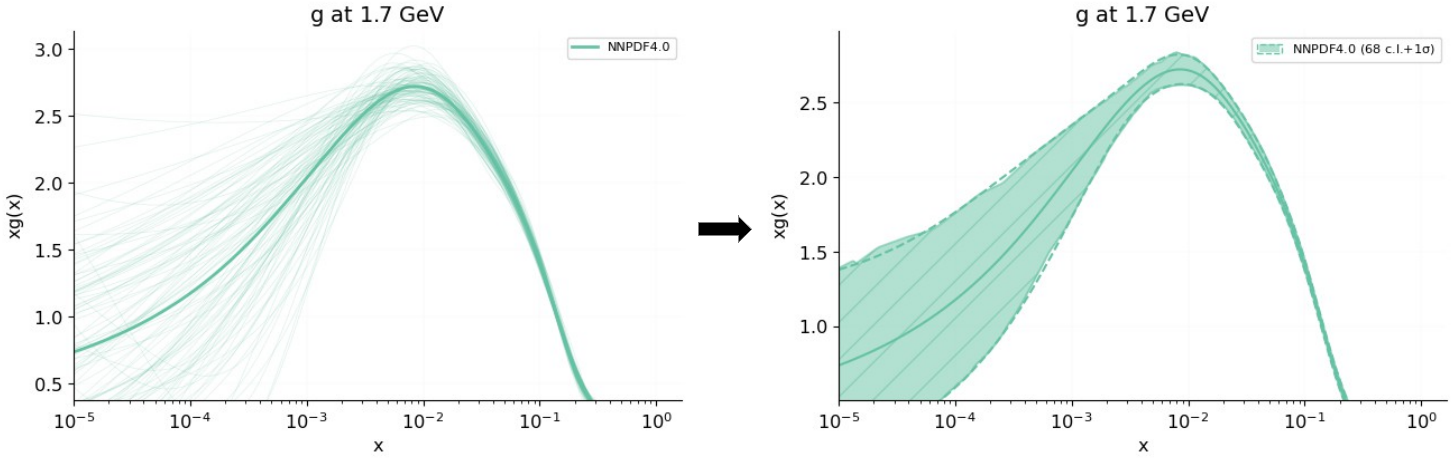
\includegraphics[width=0.7\textwidth]{intro/MC_to_uncertainty}
%Replica sample of functions $\Leftrightarrow$ Probability density in function space
\vspace*{-1cm}
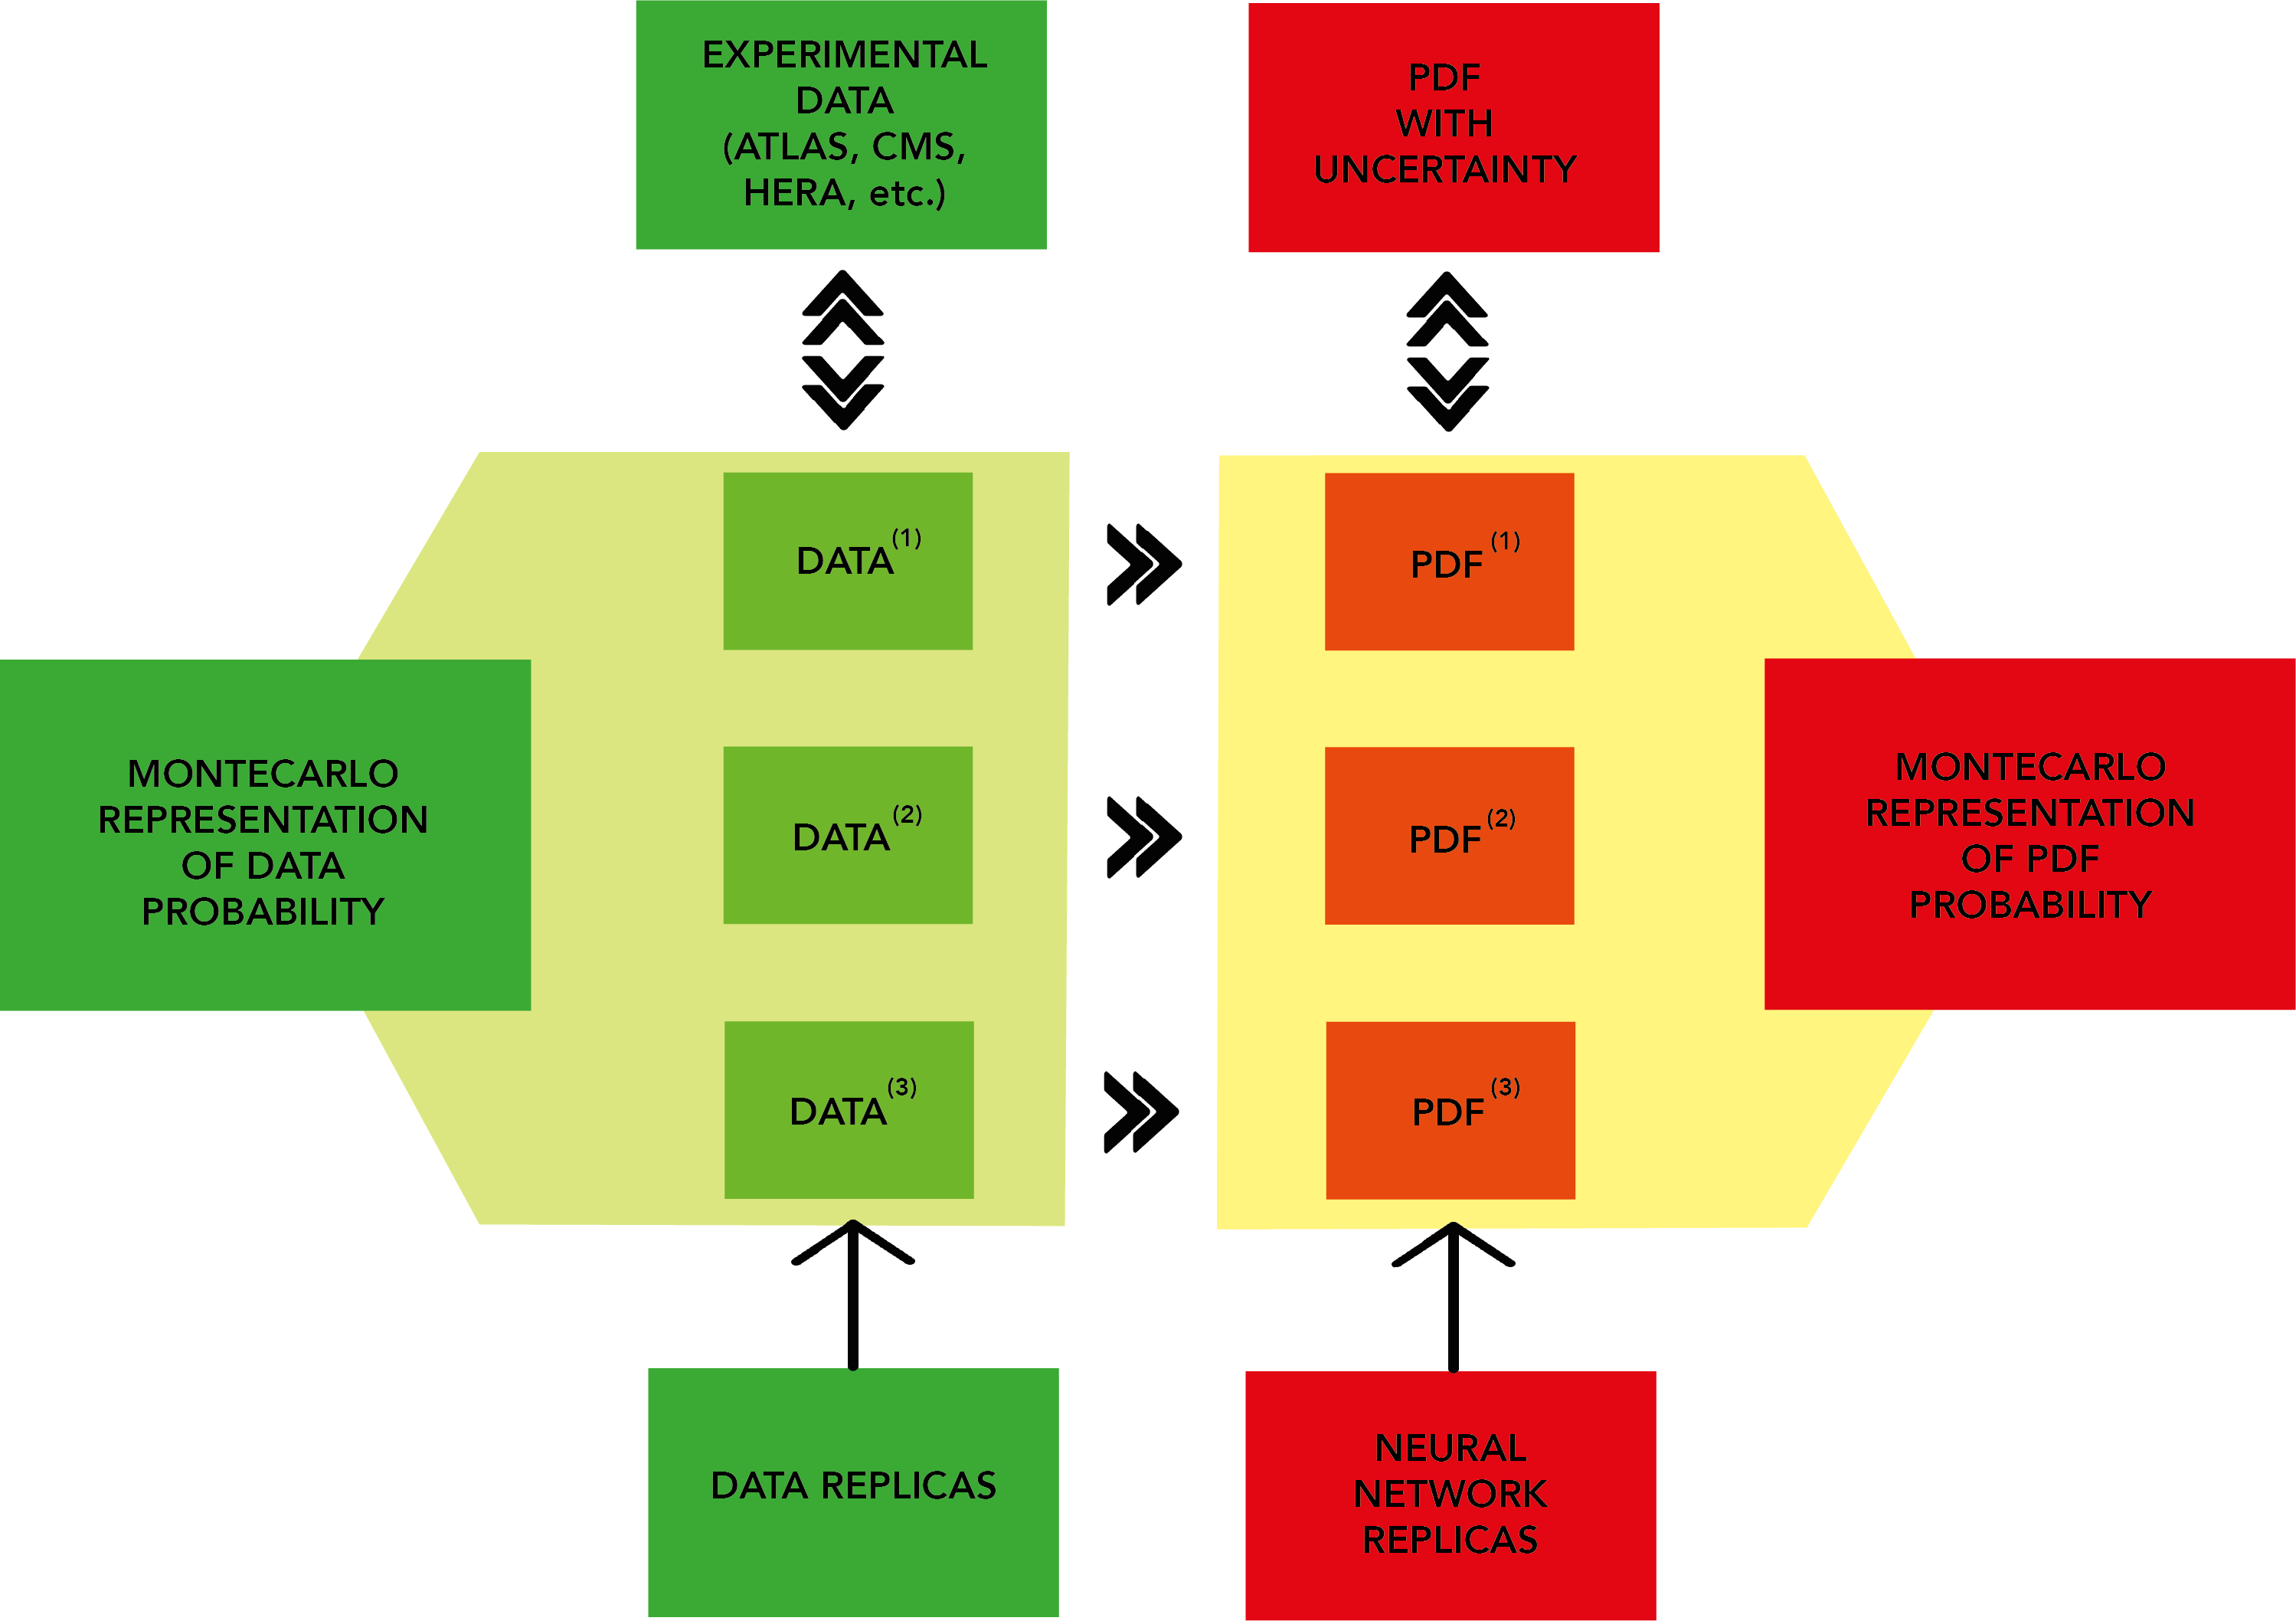
\includegraphics[width=0.5\textwidth]{intro/NNPDF_MC_strategy}
\end{center}
\end{frame}


%\begin{frame}{NNPDF3.1 methodology}
%
%The status of the methodology at time of \textbf{NNPDF3.1}:
%    \begin{itemize}
%        \item Custom \texttt{c++} code
%        \item Genetic algorithm for optimization
%        \item Manual tuning of hyperparameters
%    \end{itemize}
%
%\end{frame}


\begin{frame}[t]{Key improvements since NNPDF3.1}

%Key points of the technology used in \textbf{NNPDF3.1} addressed in this talk:
%    \begin{itemize}
%        \item Genetic algorithm for optimization
%        \item Implemented in in-house \texttt{c++} code
%        \item Manual tuning of fit parameters
%    \end{itemize}
%\vspace*{1em}

Improvements in \textbf{NNPDF4.0}:
\begin{itemize}
    \item Learning the methodology
    \begin{itemize}
        \item Systematically determine the {best model} for our data and theory
    \end{itemize}
    \item Increase {fit speed}
    \begin{itemize}
        \item Shorter fit time $\Rightarrow$ more fits
    \end{itemize}
%    \begin{itemize}
%        \item Accumulated knowledge is slow and biased
%    \end{itemize}        
%    \item Reduce \textbf{uncertainties}
%    \begin{itemize}
%        \item Phenomenological studies require an estimation of PDFs outside the data domain
%    \end{itemize}
    \item Reduction of the PDF uncertainty
    \item Validation of the {extrapolation behaviour}
%    \begin{itemize}
%        \item Testing the generalization of power the methodology
%    \end{itemize}
%    \begin{itemize}
%        \item Part of the PDF uncertainty is methodological
%    \end{itemize}
\end{itemize}
\end{frame}


%\section{Learning the methodology}
\section*{Faster fits}

\begin{frame}{NNPDF4.0 model}{For more information see  \href{https://arxiv.org/pdf/1907.05075}{\color{blue} EPJ\,C79\,(2019)\,676}}
%How can we identify the best methodology?\\
%`Accumulated knowledge' is slow and biased
\begin{figure}[t]
	\centering
	\resizebox{0.6\textwidth}{!}{%
		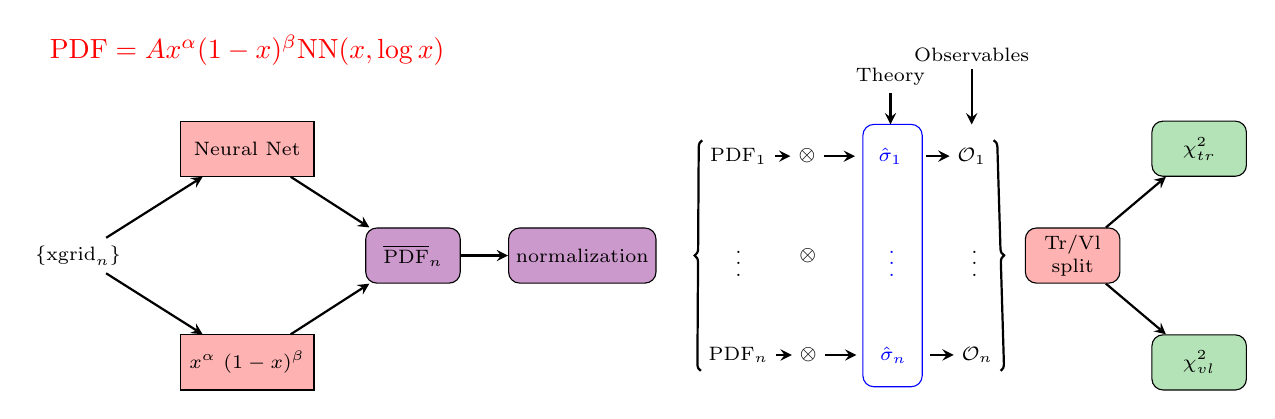
\begin{tikzpicture}[node distance = 1.0cm]\scriptsize
		% Input node
		\node (xinput) {$\{\mathrm{xgrid}_n\}$};

		% PDF basis
		\coordinate [right = 1.5cm of xinput] (NNghost) {};
		\node[fitted, above = 1.0cm of NNghost, minimum width=1.7cm, minimum height=0.7cm] (pdf) { Neural Net};
		\node[fitted, below = 1.0cm of NNghost, minimum width=1.7cm, minimum height=0.7cm] (preproc) { $x^{\alpha}$ $(1-x)^{\beta}$};
		\node[above = 0.6cm of pdf, minimum width=1.7cm, minimum height=0.3cm] (fform) 
		{\color{red} {\fontsize{10pt}{0}\selectfont $\mathrm{PDF}=Ax^\alpha(1-x)^\beta \mathrm{NN}(x,\log x)$} };

		% PDF production
		\node[operations, fill=violet!40, minimum width=1.2cm, minimum height=0.7cm, right = 1.5cm of NNghost]
		    (fitbasis) {$\overline{\mathrm{PDF}}_n$};
		\node[operations, fill=violet!40, minimum width=1.2cm, minimum height=0.7cm, right = 0.6cm of fitbasis]
		    (normalizer) {normalization};

		% PDFs 1 to n
		\node[right = 0.9cm of normalizer] (pdfdots) {\vdots};
		\node[above = 0.7cm of pdfdots] (pdf1) {PDF$_1$};
		\node[below = 0.7cm of pdfdots] (pdfn) {PDF$_n$};

		% Convolutions 1 to n
		\node[right = 0.2cm of pdf1] (conv1) {$\otimes$};
		\node[right = 0.2cm of pdfn] (convn) {$\otimes$};
		\node at ($(conv1)!0.5!(convn)$) (convdots) {$\otimes$};

		% FK Tables 1 to n
		\node[blue, right = 0.6cm of conv1] (f1) {$\hat{\sigma}_1$};
		\node[blue, right = 0.6cm of convn] (fn) {$\hat{\sigma}_n$};
		\node[blue] at ($(f1)!0.5!(fn)$) (fd) {\vdots};
		\draw[draw=blue, rounded corners] ($(f1.north west)+(-0.1, 0.2)$) rectangle ($(fn.south east)+(0.1,-0.2)$);
        \node[above = 0.6cm of f1] (theory) {Theory};
        \coordinate [above = 0.2cm of f1] (theoryarrow) {};

		% Observables
		\node[right = 0.5 cm of f1] (o1) {$\mathcal{O}_{1}$};
		\node[right = 0.5 cm of fn] (on) {$\mathcal{O}_{n}$};
		\node at ($(o1)!0.5!(on)$) (od) {\vdots};
		\node[above = 0.9cm of o1] (observables) {Observables};
		\coordinate [above = 0.2cm of o1] (observablearrow) {};

		% Tr/Vl split
		\node[operations, right = 0.5cm of od, minimum width = 1.2cm, text width=1cm, minimum height=0.7cm]
		(trvl) {Tr/Vl split};
		\coordinate [right = 1.0cm of trvl] (ending) {};
		\path let \p1 = (ending), \p2 = (pdf)
		    in node at (\x1,\y2) [n3py, minimum width = 1.2cm, minimum height=0.7cm] (tr) {$\chi^{2}_\text{tr}$};
		\path let \p1 = (ending), \p2 = (preproc)
		    in node at (\x1,\y2) [n3py, minimum width = 1.2cm, minimum height=0.7cm] (vl) {$\chi^{2}_\text{vl}$};

		% Arrows!
		\draw[myarrow] (xinput) -- (pdf);
		\draw[myarrow] (xinput) -- (preproc);
		\draw[myarrow] (pdf) -- (fitbasis);
		\draw[myarrow] (preproc) -- (fitbasis);
		\draw[myarrow] (fitbasis) -- (normalizer);

		\draw[myarrow] (pdf1) -- (conv1);
		\draw[myarrow] (pdfn) -- (convn);
		\draw[myarrow] (conv1) -- ($(f1.west)-(0.2,0.0)$) ;
		\draw[myarrow] (convn) -- ($(fn.west)-(0.2,0.0)$) ;
		\draw[myarrow] ($(f1.east)+(0.2,0.0)$) -- (o1);
		\draw[myarrow] ($(fn.east)+(0.2,0.0)$) -- (on);

		\draw[myarrow] (trvl) -- (tr);
		\draw[myarrow] (trvl) -- (vl);
		
		\draw[myarrow] (theory) -- (theoryarrow);
		\draw[myarrow] (observables) -- (observablearrow);
		
		% Braces
		\draw[decorate, decoration={brace}, thick] (pdfn.south west) -- (pdf1.north west);
		\draw[decorate, decoration={brace},thick] (o1.north east) -- (on.south east);
		\end{tikzpicture}
	}
\end{figure}
\textbf{Main changes:}
\begin{itemize}
    \item Modular \texttt{Python} codebase
        \begin{itemize}
            \item Easier and faster development
            %\item Object oriented for increased flexibility
        \end{itemize}
    \item Freedom to use external libraries (default: \texttt{TensorFlow})
%        \begin{itemize}
%            \item Gains on speed and efficiency
%            \item Use of Gradient Descent methods
%        \end{itemize}
    \item Ability to vary all aspects of the methodology
\end{itemize}

\end{frame}



%\begin{frame}[t]{Methodological differences}
%    \frametitle{Key differences with respect to the 3.1 methodology}
%    \footnotesize
%    \begin{columns}[t]
%        \column{0.5\linewidth}
%            \mycolutitle{NNPDF 3.1 code}
%            \begin{list}{\color{darkred} $\rightarrow$}{}
%                \item C++ monolithic codebase
%                 \item In-house Machine Learning \\ optimization framework
%                \item Genetic Algorithm optimizer
%                \item One network per flavour
%                \item Fitting times of up to several days
%                \item  Genetic Algorithm optimizer
%                 \item Fit parameters manually chosen
%            \end{list}
%        \column{0.5\linewidth}
%            \mycolutitle{NNPDF 4.0 code}
%            \begin{list}{\color{darkgreen} $\rightarrow$}{} 
%                \item Python modular codebase 
%                \item Freedom to use external libraries \\ (default: \texttt{TensorFlow})
%                \item Gradient Descent optimization
%                \item One network for all flavours
%                \item Results available in about an hour
%                \item Gradient Descent optimization
%                 \item Fit parameters chosen automatically (hyperparameter scan)
%            \end{list}
%    \end{columns}
%\end{frame}


\begin{frame}{Improved performance}
\begin{table}
   \renewcommand{\arraystretch}{1.50}
	\centering
	\begin{tabular}{c | c | c | c} \toprule
	  & NNPDF3.1  & NNPDF4.0 (CPU) & NNPDF4.0  (GPU) \\
          \midrule
	  Fit timing per replica    & 15.2 h        & 38 min        & 6.6 min \\ \hline
           Speed up factor    & 1        &  24      & 140 \\ \hline
	  RAM use &  1.5 GB          &  6.1 GB                 & NA  \\ \bottomrule
	\end{tabular}
\end{table}
\vspace*{1em}
\textbf{Benefits}:
    \begin{itemize}
        \item Fewer CPU hours for a fit
        \item Use of gradient descent optimization $\Rightarrow$ more stable results\\
        \vspace*{1em}
        \item[$\Rightarrow$] Possibility to learn the methodology
    \end{itemize}
    
%    \begin{itemize}
%        \item \textbf{Fewer CPU hours} to obtain a fit
%        \begin{itemize}
%            \item[$\Rightarrow$] Try more parameter configurations in less time
%            \begin{itemize}
%                \item[$\Rightarrow$] Possible to automatically learn the methodology
%            \end{itemize}
%        \end{itemize}
%    \end{itemize}
\end{frame}

\section*{Learning the methodology}

\begin{frame}{Finding the best methodology: hyperoptimization}

\begin{center}
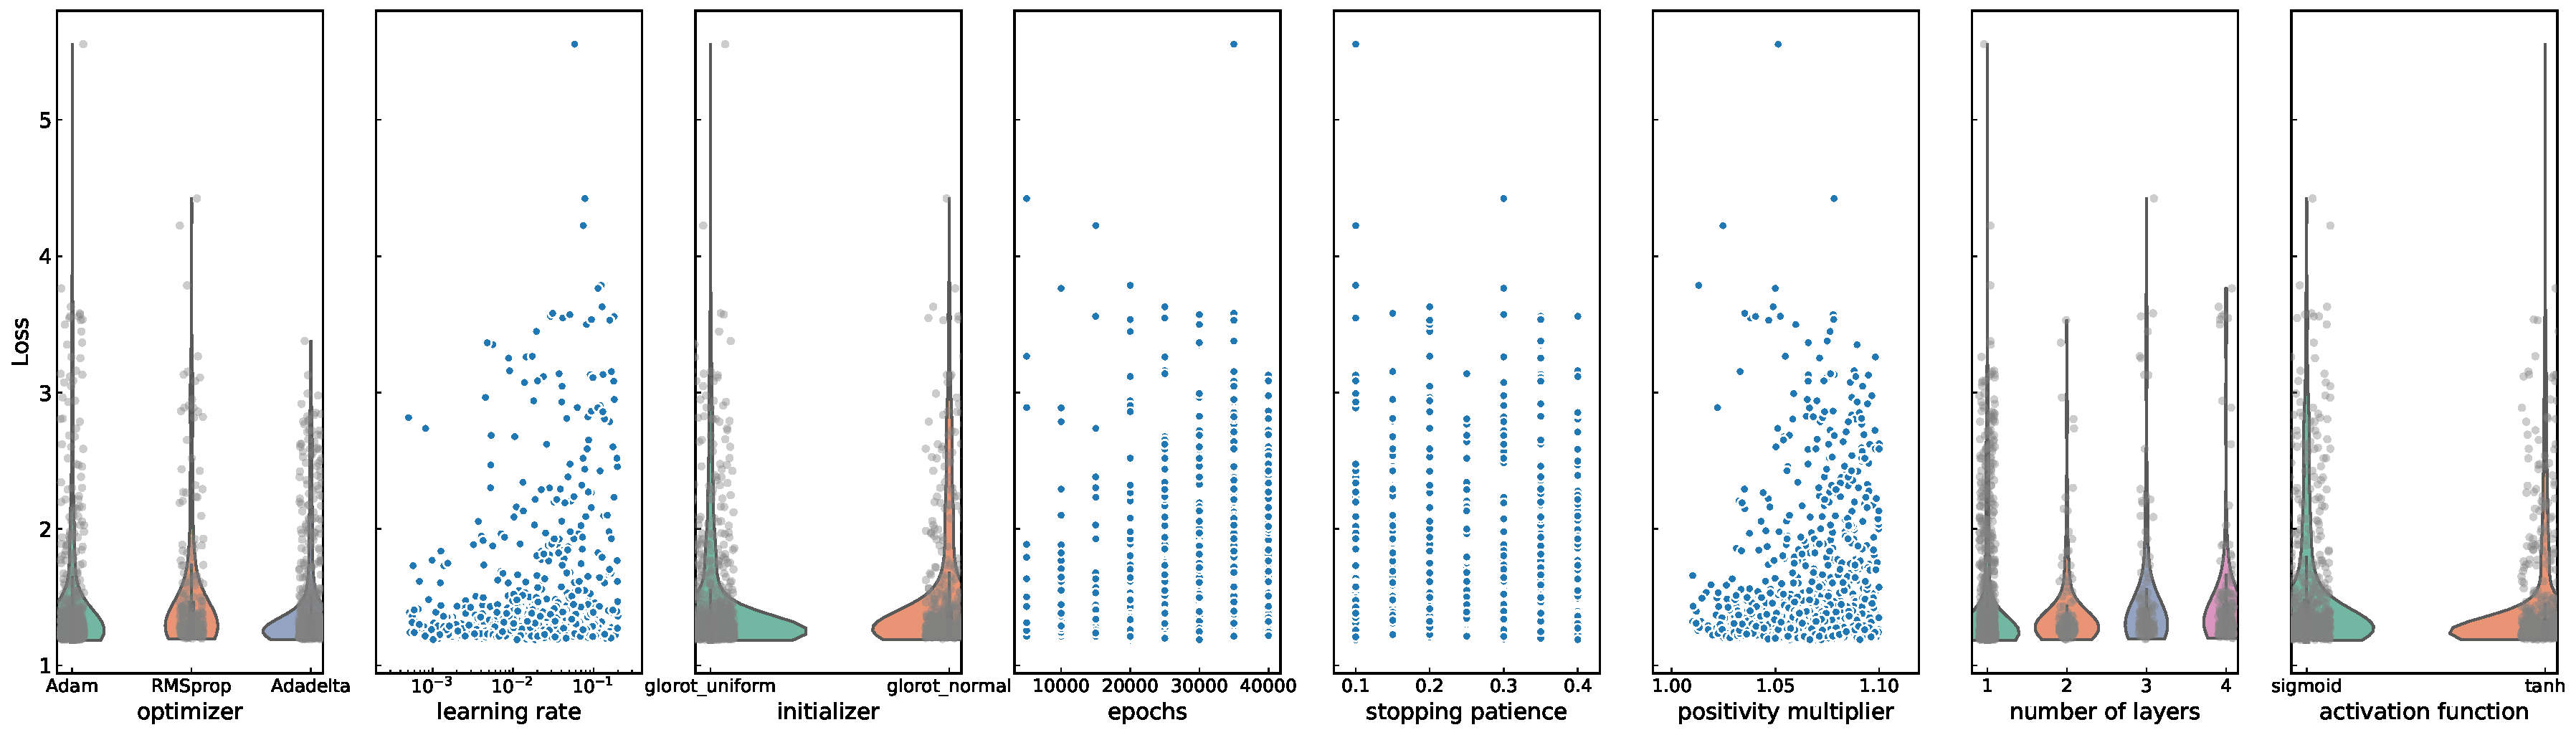
\includegraphics[width=0.9\textwidth]{methodology/hyperopt_scan}
\end{center}
    \begin{itemize}
        \item \textbf{Scan} parameter space
        \item \textbf{Optimize} figure of merit: validation $\chi^2$
        %\item Use \textbf{Bayesian} updating (\texttt{hyperopt})
    \end{itemize}
\end{frame}



\begin{frame}{Overfitting}
Using the validation set $\chi^2$ as figure of merit leads to overfitting:
\begin{center}
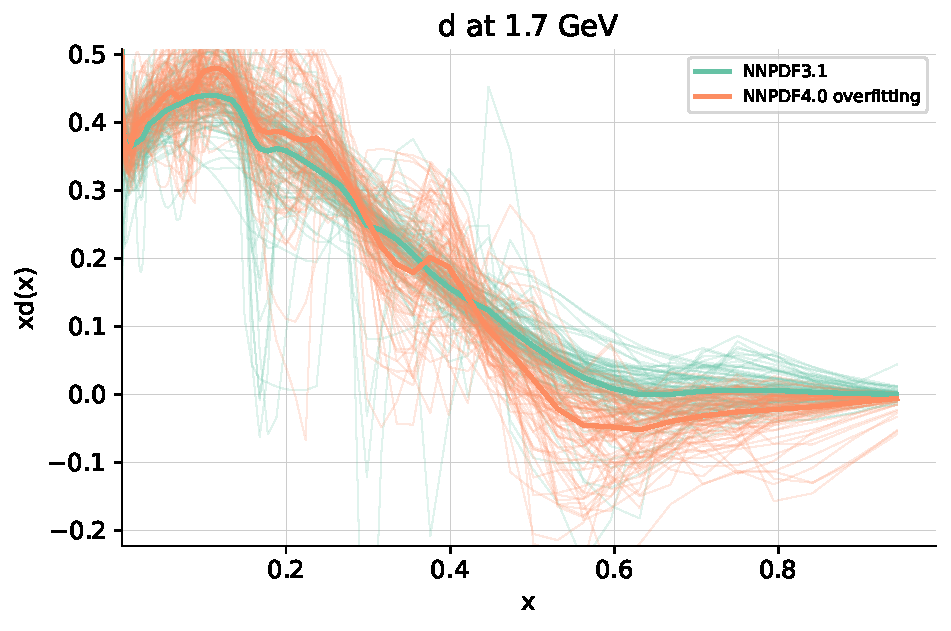
\includegraphics[width=0.4\textwidth]{methodology/overfit_nnpdf31}
\end{center}
    \begin{itemize}
        \item NNPDF3.1: wiggles are a \textbf{finite size effect} that vanishes as $N_\mathrm{rep}$ grows
        \item NNPDF4.0: genuine \textbf{overfitting} with $\chi^2_\mathrm{train} \ll \chi^2_\mathrm{val}$
%        \item NNPDF4.0: genuine \textbf{overfitting} due to training-validation data correlations
%        \vspace*{0.5em}
%        \item[$\Rightarrow$] Define a proper quality control
    \end{itemize}
\end{frame}

\begin{frame}{What happened?}
\centering
    \textbf{Correlations} between training and validation data \\
    \begin{figure}
        \centering
        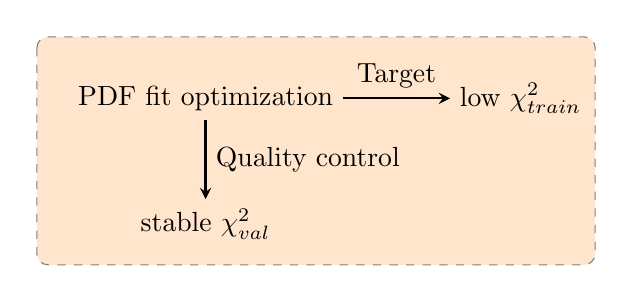
\begin{tikzpicture}[node distance = 4.0cm] 
            \node (a) {PDF fit optimization};
            \node [below = 1cm of a] (b) {stable $\chi^{2}_{\text{val}}$};
            \node [right of = a] (c) {low $\chi^{2}_{\text{train}}$};
            \draw[arrow] (a) -- node [right, midway] {Quality control} (b);
            \draw[arrow] (a) -- node [above, midway] {Target} (c);

            \begin{pgfonlayer}{bg}
                \path (a.north west) + (-0.4, 0.5) node (ab) {};
                \path (b.south east) + (+4.0,-0.2) node (bb) {};
                
                \path[fill=orange!20,rounded corners, draw=black!50, dashed]
                    (ab) rectangle (bb);           
            \end{pgfonlayer}
        \end{tikzpicture}
    \end{figure}
    $\Rightarrow$ Define a proper quality control!
\end{frame}


\begin{frame}{Removing overfitting: the test set}
\centering
    Define an uncorrelated {\color{red} test set} to test generalization power on unseen data\\
    \begin{figure}
        \centering
        	\resizebox{0.6\textwidth}{!}{%
        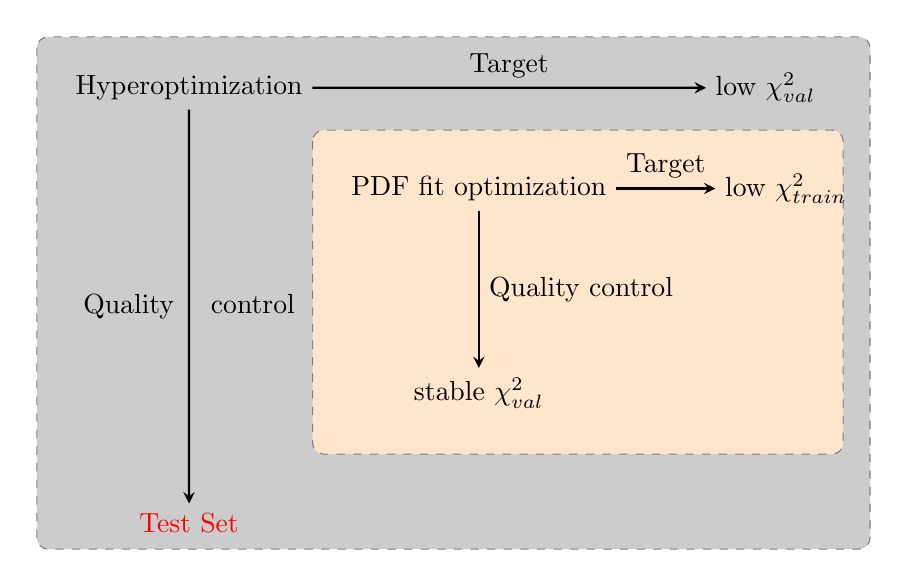
\begin{tikzpicture}[node distance = 3.9cm, scale = 0.92] 
            \node (a) {PDF fit optimization};
            \node [below = 2cm of a] (b) {stable $\chi^{2}_{\text{val}}$};
            \node [right of = a] (c) {low $\chi^{2}_{\text{train}}$};
            \draw[arrow] (a) -- node [right, midway] {Quality control} (b);
            \draw[arrow] (a) -- node [above, midway] {Target} (c);

            \coordinate (e) at ( $(a) + (-4.0, 0.0)$ );
            \node (f) [above = 1.0cm of e] {Hyperoptimization};
            \node (g) [right = 5cm of f] {low $\chi^{2}_{\text{val}}$};
            \node (h) [below = 5cm of f] {\color{red} Test Set};
            \draw[arrow] (f) -- node [above, midway] {Target} (g);
            \draw[arrow] (f) -- node [midway] {Quality \ \ \ control} (h);

            \begin{pgfonlayer}{bg}
                \path (f.north west) + (-0.4, 0.4) node (fb) {};
                \path (h.south) + (+9.4,-0.1) node (hb) {};
                \path[fill=black!20,rounded corners, draw=black!50, dashed]
                    (fb) rectangle (hb);           

                \path (a.north west) + (-0.4, 0.5) node (ab) {};
                \path (b.south east) + (+4.0,-0.5) node (bb) {};
                \path[fill=orange!20,rounded corners, draw=black!50, dashed]
                    (ab) rectangle (bb);           
            \end{pgfonlayer}
        \end{tikzpicture}
        }
    \end{figure}

\end{frame}


\begin{frame}{Removing overfitting: k-fold cross-validation}
\begin{columns}
\column{0.48\linewidth}
The basic idea of \textbf{k-fold cross-validation}:
\begin{enumerate}
    \item Divide the data into $k$ {representative subsets}
    %\item \label{ite:2} Pick a hyperparameter setup
    \item Fit $k-1$ sets and use $k$-th as test set
    \begin{itemize}
        \item[$\Rightarrow$] $k$ values of $\chi^2_\mathrm{test}$
    \end{itemize}
    \item Optimize the average $\chi^2_\mathrm{test}$ of the $k$ test sets
\end{enumerate}


\column{0.48\linewidth}
%Using k-fold cross-validation for model selection:

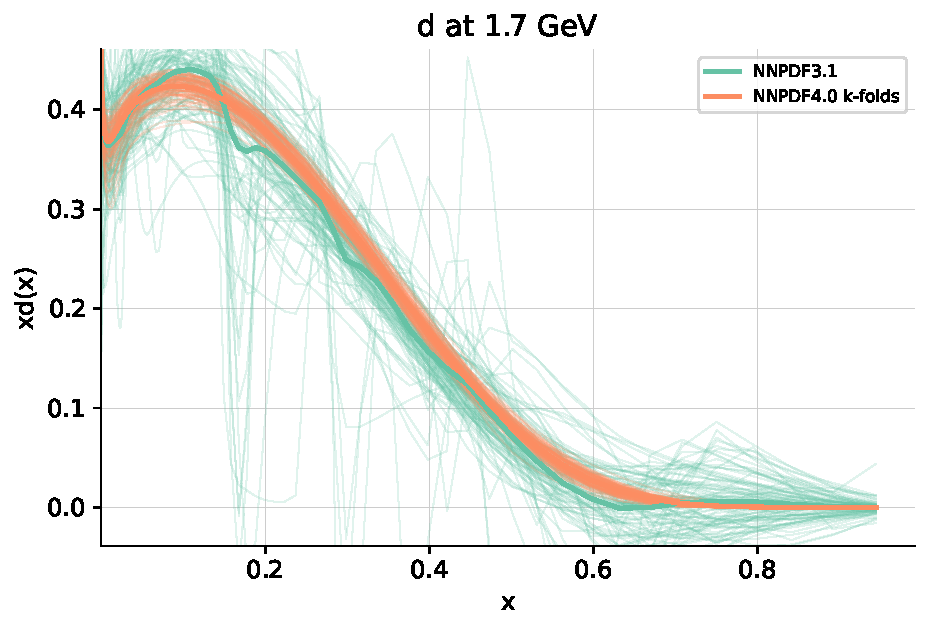
\includegraphics[width=0.8\textwidth]{methodology/best_model_vs_nnpdf31}

\begin{itemize}
     \item No overfitting\\
     \vspace*{0.2em}
     \item Compared to NNPDF3.1:
    \begin{itemize}
        \item Increased stability
        \item Reduced uncertainties 
    \end{itemize}
\end{itemize}


\end{columns}
\end{frame}




%\section{Uncertainty validation}
\section*{Validating extrapolation}

\begin{frame}{Trusting uncertainties outside the data region}

\begin{itemize}
        \item The improved methodology and extended dataset result in a reduction of the PDF uncertainties.
        \item Can we trust the uncertainties in the extrapolation region?
\end{itemize}

\begin{columns}
    \column{0.48\linewidth}
    \textbf{Idea:}
    \begin{enumerate}
    \item Take a historic dataset \\ e.g. pre-HERA or pre-LHC
    \item Perform fit
    \item Compare predictions to ``future'' data
    \end{enumerate}

    \column{0.48\linewidth}
     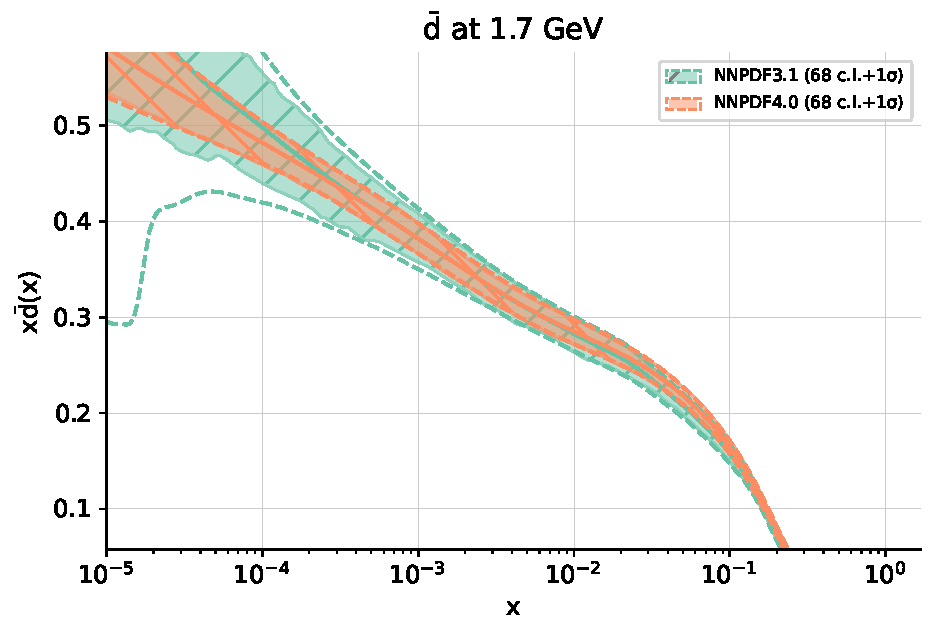
\includegraphics[width=0.9\textwidth]{future_test/NNPDF31_vs_NNPDF40}
\end{columns}
\end{frame}


\begin{frame}[t]{Future tests}{For more information see \href{https://arxiv.org/pdf/2103.08606.pdf}{\color{blue} arxiv:2103.08606}}

    \begin{columns}
        \column{0.60\linewidth}
        \centering
        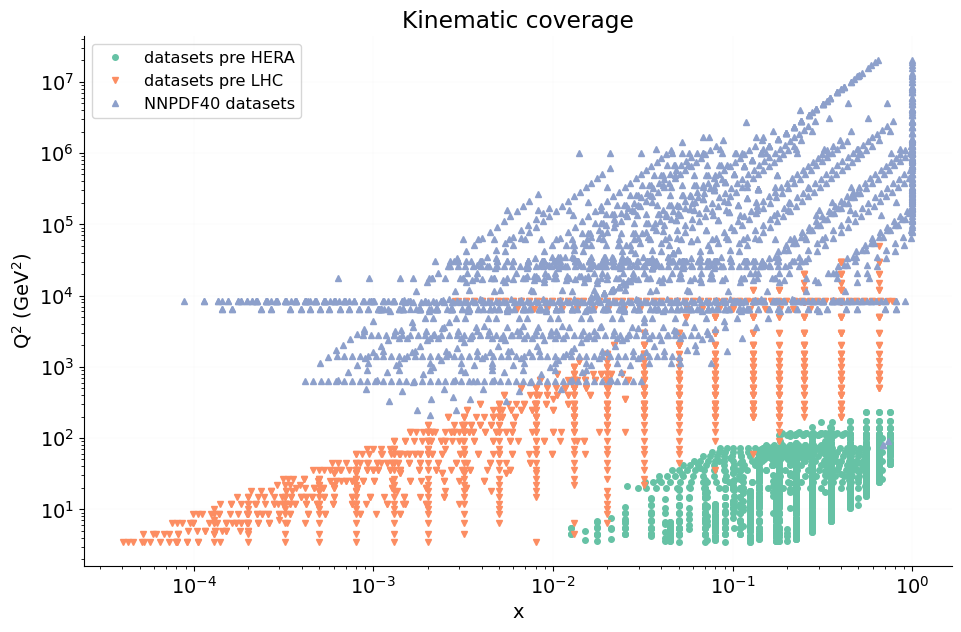
\includegraphics[width=0.8\textwidth]{future_test/kincov.png}
        \column{0.46\linewidth}
        \vspace{-1.7cm}
        \only<1>{
            \begin{table}
                \tiny
                \centering
                \caption*{\scriptsize $\chi^{2}/N$ (only exp. covmat)}
                \begin{tabular}{c | c c c} \toprule
                    (dataset) & NNPDF4.0 & pre-LHC & pre-Hera  \\ \midrule
                    pre-HERA  & 1.09 & 1.01 & 0.90 \\
                    pre-LHC   & 1.21 & 1.20 & \hlme{23.1} \\
                    NNPDF4.0  & 1.29 & \hlme{3.30} & \hlme{23.1} \\
                    \bottomrule
                \end{tabular}
            \end{table}
        }
        \only<2>{
            \begin{table}
                \tiny
                \centering
                \caption*{\scriptsize $\chi^{2}/N$ (exp. and PDF covmat)}
                \begin{tabular}{c | c c c} \toprule
                    (dataset) & NNPDF4.0 & pre-LHC & pre-Hera  \\ \midrule
                    pre-HERA  &  & & 0.86 \\
                    pre-LHC   &  & 1.17 & \hlme{1.22} \\
                    NNPDF4.0  & 1.12 & \hlme{1.30} & \hlme{1.38} \\
                    \bottomrule
                \end{tabular}
            \end{table}
        }


        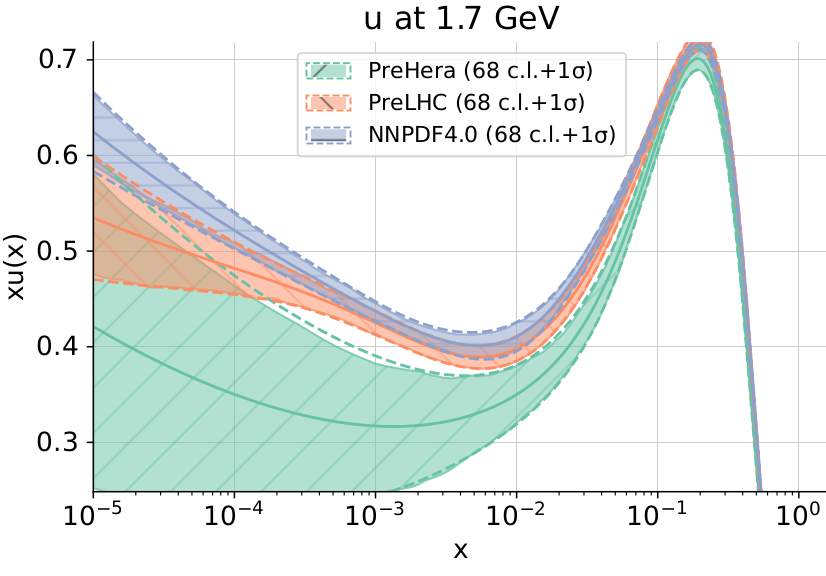
\includegraphics[width=0.9\textwidth]{future_test/diffu}
    \end{columns}
        \only<2>{\small The total uncertainty increases, and accommodates for difference between predictions and new data.}
\end{frame}


%
%\section{Methodology correlations}
%
%\begin{frame}{Self-correlation of PDF sets}
%    	\begin{columns}[t]
%        	\column{0.58\linewidth}
%        	\vspace*{-0.8cm}
%        	
%		 Is the data-induced correlation between PDF sets based on the same NNPDF methodology and underlying data 100\%?
%
%        	\vspace{0.2cm}
%
%        \begin{block}{data-induced correlation}
%        Data-induced correlation is calculated using PDF pairs fitted to the same data replicas.
%        \end{block}
%        	
%        	\vspace{0.2cm}
%
%			No, the data-induced correlation is not 100\%. This is a result of uncorrelated functional uncertainties.
%
%		\vspace{0.2cm}
%			\only<2>{If the data-induced correlation is higher, this means the functional uncertainty is smaller if compared to the data uncertainty.}
%
%        	\column{0.38\linewidth}
%        	\vspace*{-1cm}
%        		\begin{center}
%        		\begin{figure}
%            		\includegraphics<1>[width=\textwidth]{corr/nnpdf31_corr.pdf}
%            		\includegraphics<2>[width=\textwidth]{corr/nnpdf31&40_corr.pdf}
%            		\vspace{-0.9cm}
%            		\caption{\tiny PDF-PDF self-correlation between two PDF sets based on the same NNPDF methodology and data, but different (random) initialization. }        		
%			\end{figure}
%			\end{center}
%
%    	\end{columns}
%\end{frame}
%
%
%\begin{frame}{Combination of PDF sets}
%    	\begin{columns}[t]
%        	\column{0.58\linewidth}
%
%			At present the PDF4LHC combination method is a simple averaging. 
%
%        	\vspace{0.2cm}
%
%			Can we achieve a more precise results by including underlying data-induced correlations?
%
%        	\vspace{0.2cm}
%
%			No, this can lead to arbitrarily small uncertainties.
%
%       	\column{0.38\linewidth}
%       	\vspace{-1.5cm}
%       	\begin{center}
%       		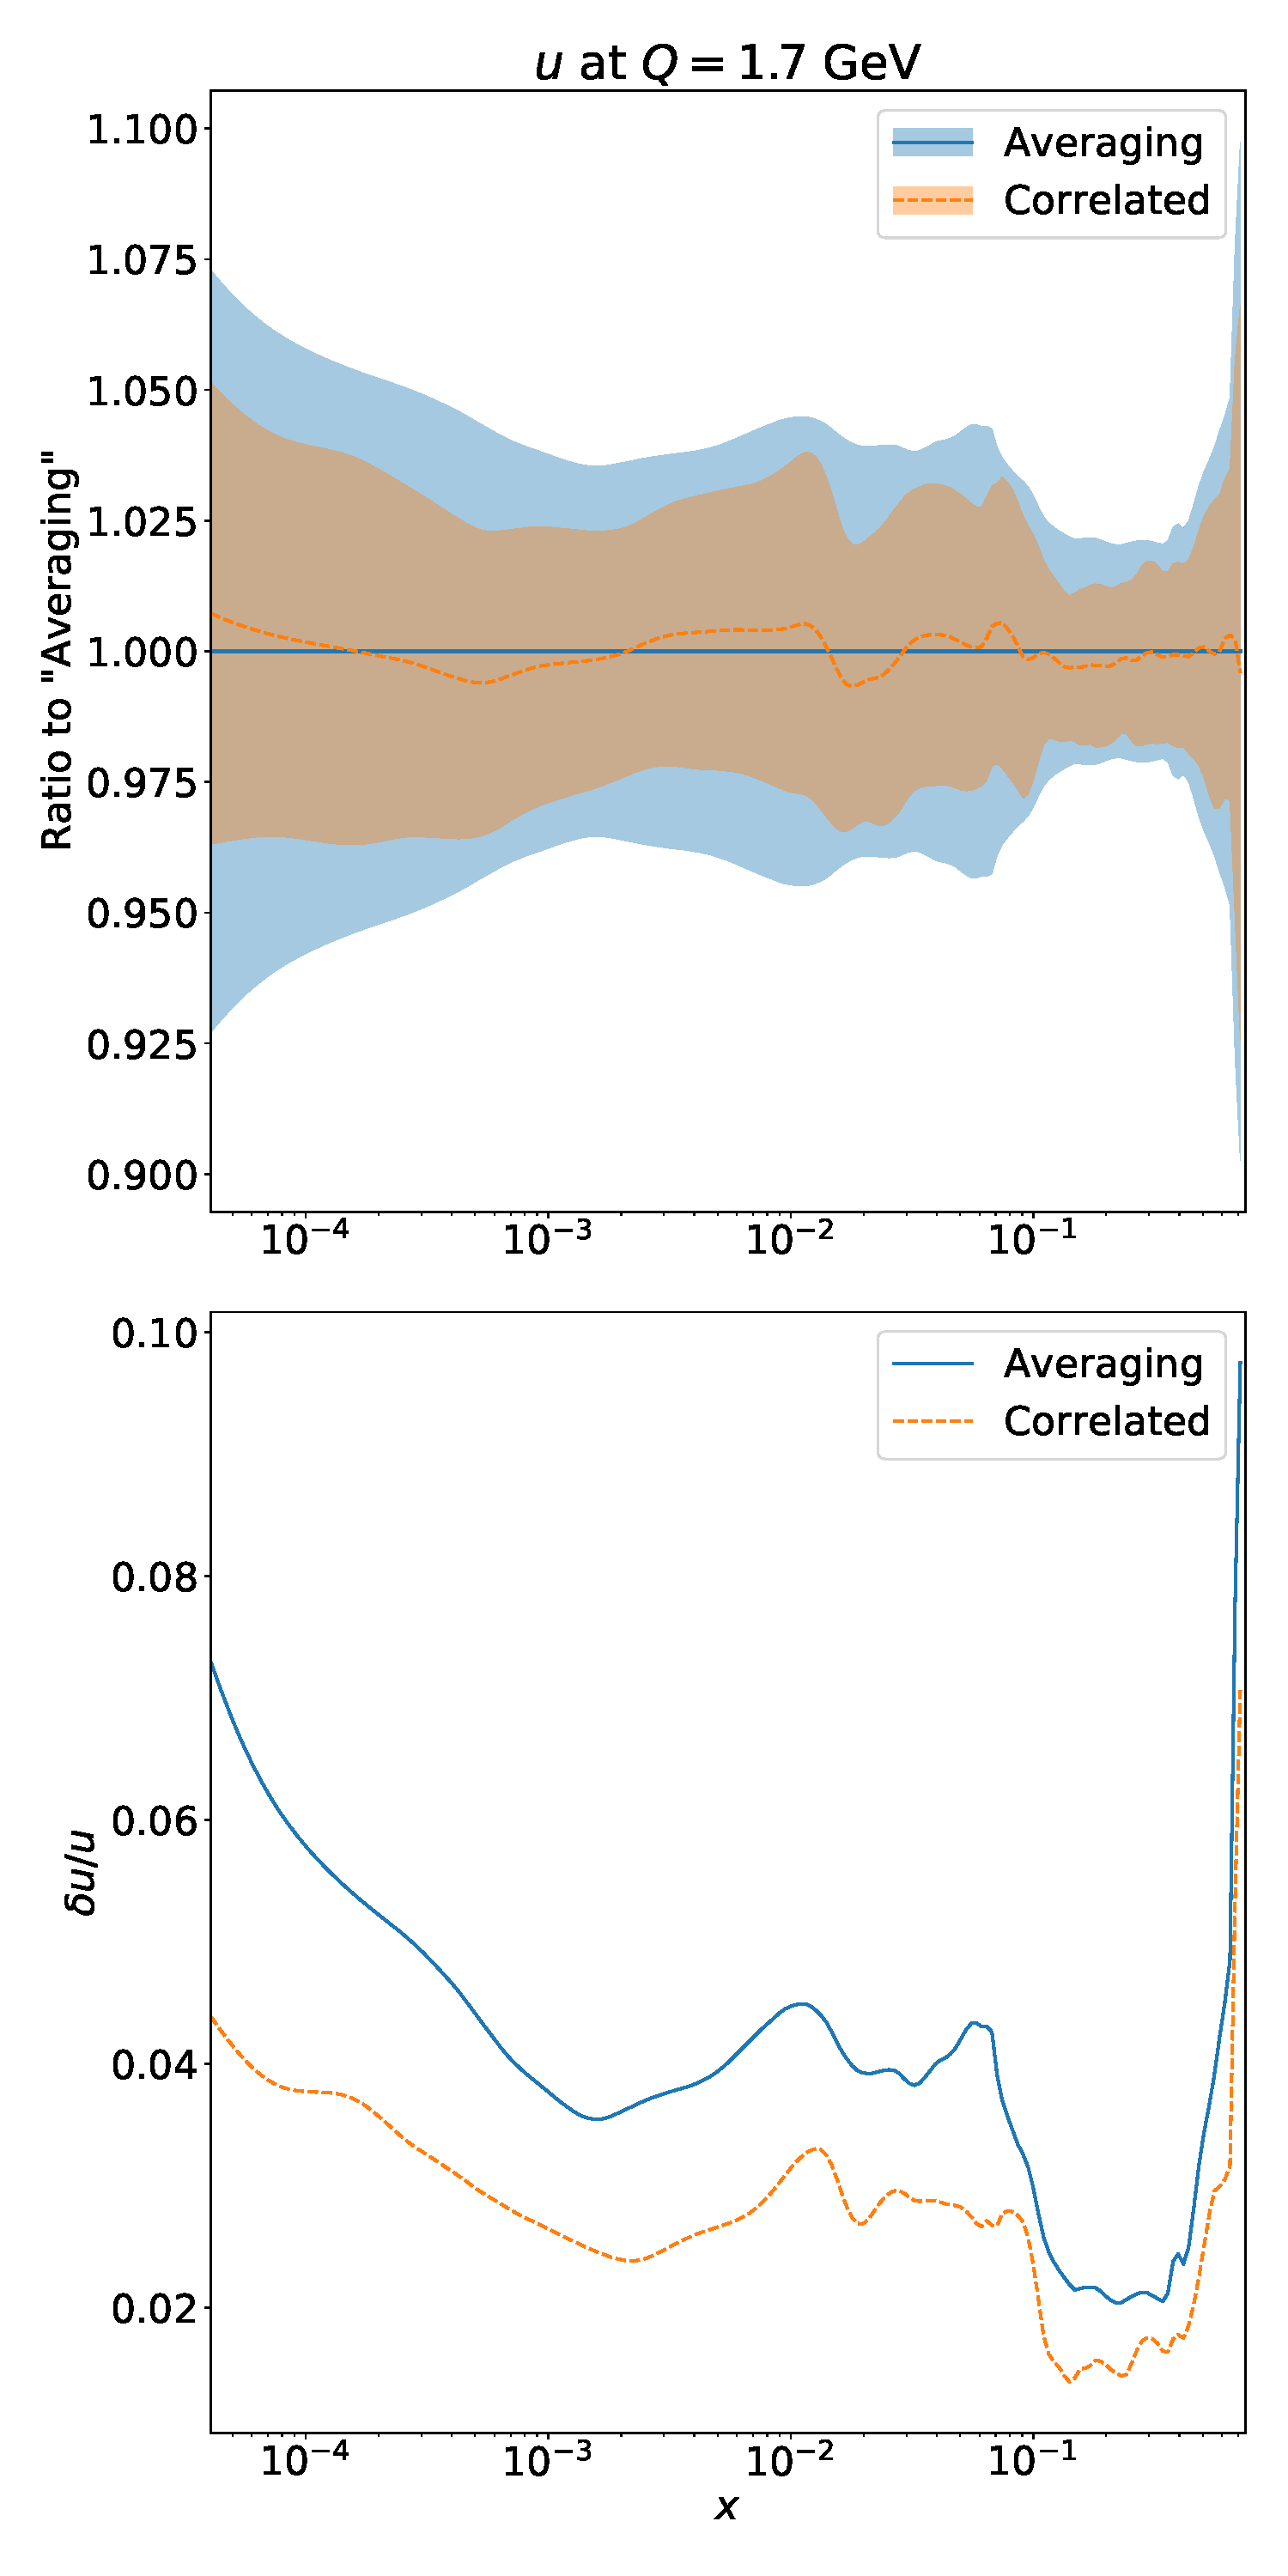
\includegraphics[height=0.9\textheight]{corr/ratio_2.pdf}
%       	\end{center}
%			
%    	\end{columns}
%\end{frame}




\section{Future challenges}

\begin{frame}{Preprocessing}
\begin{columns}[t]
\column{0.58\linewidth}

The current model parametrization uses \textbf{preprocessing}:\\
$\mathrm{PDF}=x^\alpha(1-x)^\beta \mathrm{NN}({x,\log x})$

\vspace*{0.2cm}
If preprocessing is removed, we observe freezing at small-x:
\begin{center}
$\mathrm{PDF}= \mathrm{NN}(x)$ \\
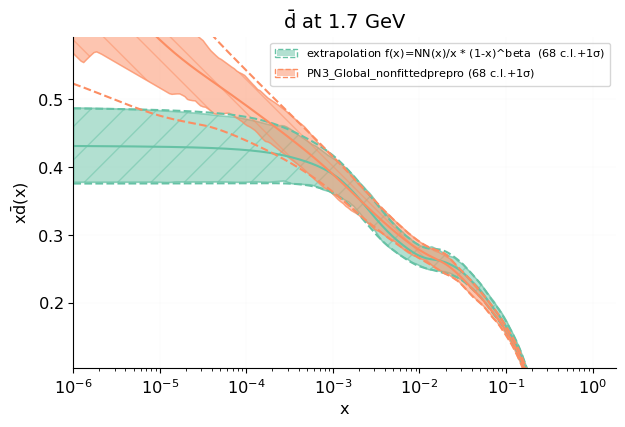
\includegraphics[width=0.48\textwidth]{feature_scaling/flatdbar}
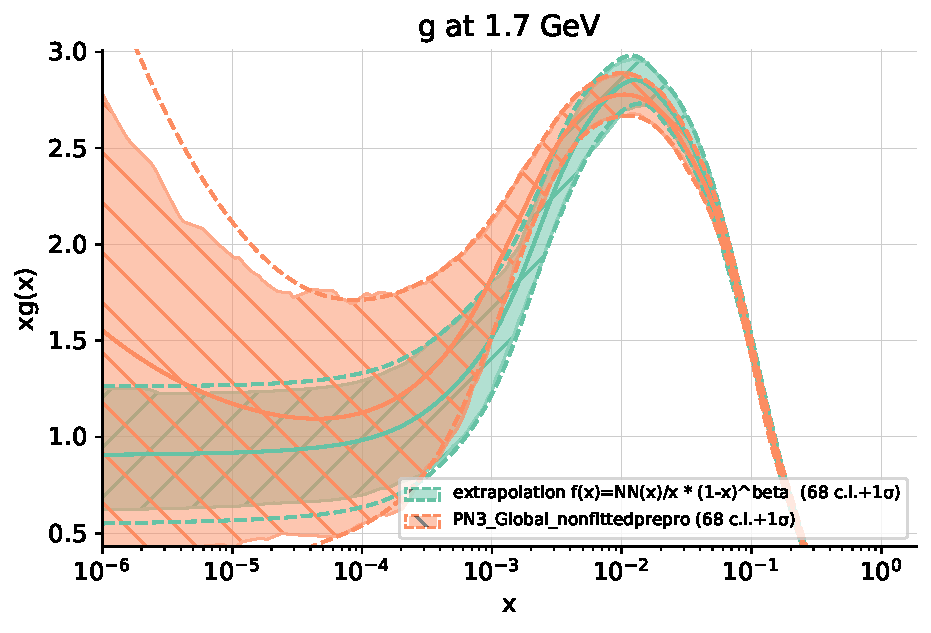
\includegraphics[width=0.48\textwidth]{feature_scaling/gluon_saturation}
\end{center}

\column{0.38\linewidth}
\textbf{Challenges:}
\begin{itemize}
    \item Modify the {neural network} \\ \textbf{input architecture}
    \item Generate {pseudodata} in the \textbf{extrapolation region}
\end{itemize}

\end{columns}
\end{frame}



\begin{frame}{Modify the input}
\begin{columns}
\column{0.58\linewidth}
Solution:
\begin{enumerate}
\item<1-|alert@1-2> Scale the input such that it is homogeneously distributed
\item<1-|alert@3> Select one in $n$ points  
\item<1-|alert@4> Provide a monotonically increasing interpolation
\end{enumerate}

\only<1-4>{{ Result: $\mathrm{PDF}=\left(\text{NN}(x')-\text{NN}(1)\right)$}}
%\only<5>{\alert{ Result: $\mathrm{PDF}={A} \text{NN}(x')$}}
\only<5>{\alert{ Result: $\mathrm{PDF}= \left(\text{NN}(x')-\text{NN}(1)\right)$}}

\column{0.38\linewidth}
\only<5>{\\
\textbf{Pro:} removed $x$, $\log x$\\
\textbf{Con:} no control in the extrapolation region
}
\end{columns}

% figures of xgrid histogram, or maybe simple example of 1D grid of points
\begin{center}
\only<1>{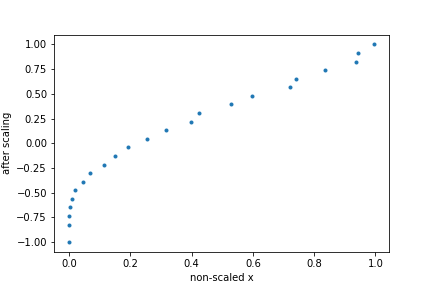
\includegraphics[height=0.25\textwidth]{feature_scaling/feature_scaling_1}}
\only<2>{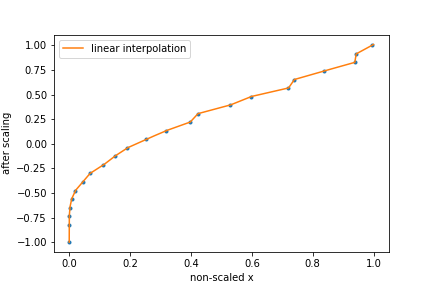
\includegraphics[height=0.25\textwidth]{feature_scaling/feature_scaling_2}}
%\only<3>{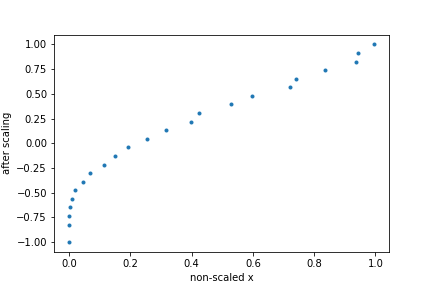
\includegraphics[height=0.3\textwidth]{feature_scaling/feature_scaling_1}}
\only<3>{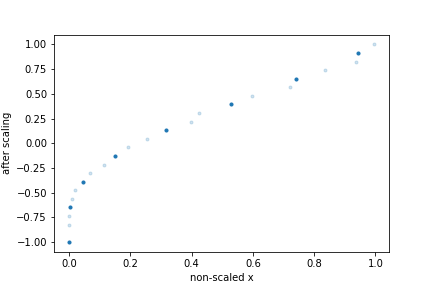
\includegraphics[height=0.25\textwidth]{feature_scaling/feature_scaling_3}}
\only<4>{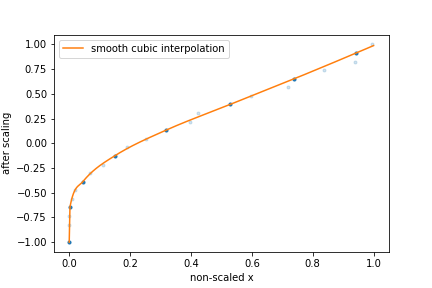
\includegraphics[height=0.25\textwidth]{feature_scaling/feature_scaling_4}}
\only<5>{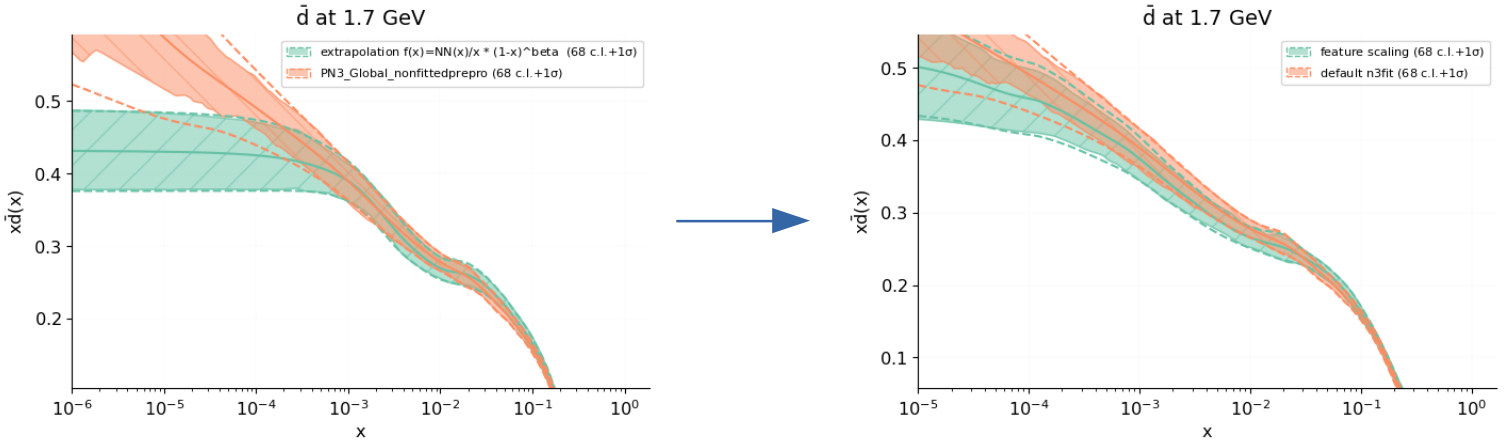
\includegraphics[height=0.25\textwidth]{feature_scaling/flat_to_feature}
}
\end{center}

\end{frame}


\begin{frame}{ The extrapolation region}
\begin{columns}
\column{0.58\linewidth}
    \textbf{Idea:}
    \begin{enumerate}
        \item Use {Gaussian Process} to model {DIS observables}
        \item Propagate a Gaussian prior into the {extrapolation region}
        \item Generate {Gaussian pseudodata} and include in in a fit
    \end{enumerate}
\column{0.38\linewidth}
    \textbf{Challenges:}
    \begin{itemize}
        \item Large uncertainty $\Rightarrow$ low weight in $\chi^2$
        \item Generating {accurate predictions}
    \end{itemize}
\end{columns}
        \begin{center}
            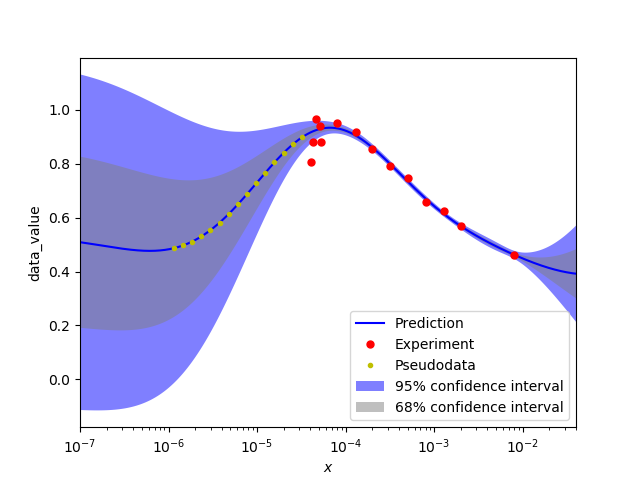
\includegraphics[width=0.35\textwidth]{feature_scaling/GP}
            %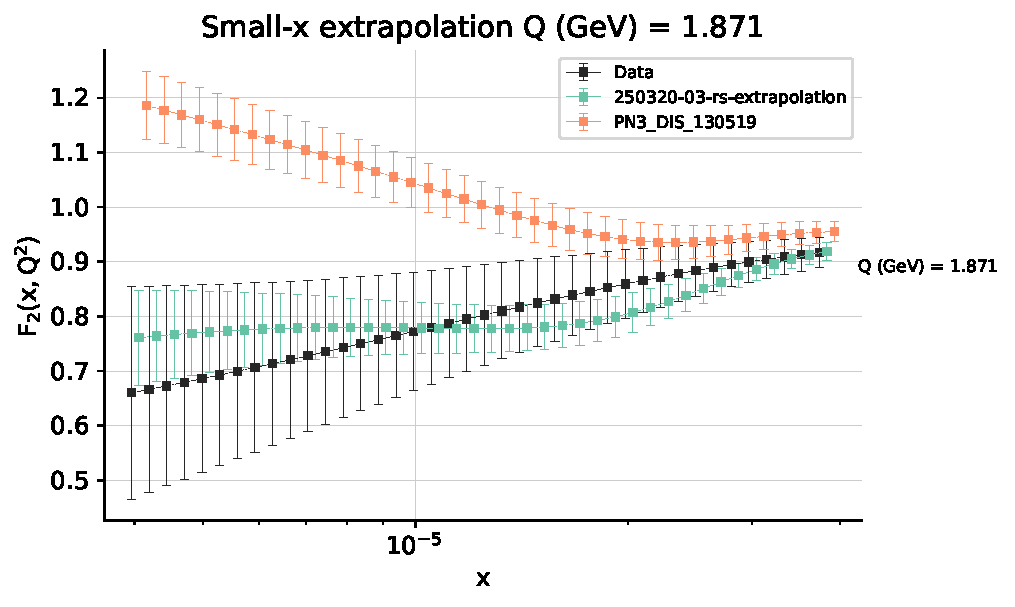
\includegraphics[width=0.45\textwidth]{feature_scaling/DIS_pseudodata}
        \end{center}
\end{frame}


\section*{Conclusions}


\begin{frame}{Summary}
    \begin{itemize}
        \item Faster and more stable results
        \item Possibility to learn the methodology 
        \item Faithful reduction of uncertainties
        %\item Correlations can be used to assess the efficiency of the methodology
        \vspace*{1em}
        \item NNPDF code will be made publicly available with documentation
    \end{itemize}
\end{frame}




\begin{frame}{Determination of the photon PDF}
  \begin{columns}[T]
    \begin{column}{0.59\textwidth}
      Initially the photon PDF has been determined in different ways:
      \begin{itemize}
        \item physical model: sensitive to underlying model
        \item fitting: data does not provide strong constraints
      \end{itemize}

      \vspace*{0.5em}
      However with the LUXqed approach it can be computed perturbatively \\
      based on the observation that the heavy-lepton production cross-section can be written in two ways:
      \begin{itemize}
        \item in terms of structure functions $F_2$, $F_L$
        \item in terms of PDFs (including the photon)
      \end{itemize}

      \vspace*{0.5em}
      luxQED result {\color{gray}\small[Manohar, Nason, Salam, Zanderighi: 1607.04266, 1708.01256]}:
      \vspace*{-0.8em}
      \begin{equation*}
        \begin{split}
          & x \gamma(x, \mu^2)
          =
          \frac{2}{\alpha (\mu^2)} \int\limits_x^1 \frac{dz}{z}
          \Biggl\{ \int_{m_p^2x^2 \over 1-z}^{\mu^2 \over 1-z} \frac{dQ^2}{Q^2}
          \alpha^2(Q^2) \Biggl[ -z^2 F_L(x/z, Q^2) \\
          & + \left( z P_{\gamma q}(z) + \frac{2 x^2 m_p^2}{Q^2} \right)
          F_2(x/z, Q^2)\Biggr] - \alpha^2(\mu^2) z^2 F_2(x/z, \mu^2)\Biggr\}
        \end{split}
      \end{equation*}
    \end{column}

    \begin{column}{0.39\textwidth}
      \vspace*{-2.5em}
      \begin{figure}
        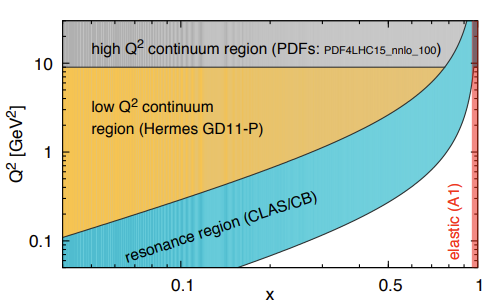
\includegraphics[width=0.89\textwidth]{figures/dataluxqed.png}
        \caption*{Input to construct $F_2$ and $F_L$}
        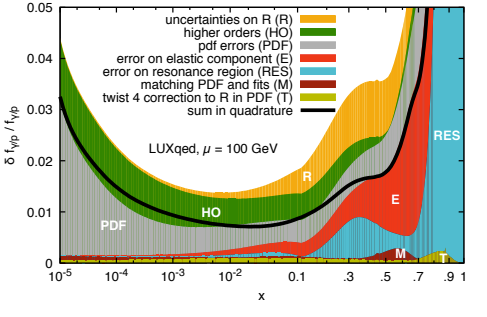
\includegraphics[width=0.89\textwidth]{figures/luxQED_uncs.png}
        \caption*{Sources of uncertainty}
      \end{figure}
    \end{column}
  \end{columns}
\end{frame}


\begin{frame}{LUXqed PDF determinations}
  LUXqed has been used in all of the most recent QED PDFs:
  \begin{itemize}
      \item LUXqed\_plus\_PDF4LHC15 {\color{gray}\small [1607.04266]}
      \item LUXqed17\_plus\_PDF4LHC15 {\color{gray}\small [1708.01256]}
      \item MMHT2015qed {\color{gray}\small [1907.02750]}
      \item NNPDF3.1luxQED {\color{gray}\small [1712.07053]}
      \item CT18lux and CT18qed {\color{gray}\small [2106.10299]}
      \item MSHT20QED {\color{gray}\small [2111.05357]}
      \item MSHT20qed\_an3lo {\color{gray}\small [2312.07665]}
      \item NNPDF4.0QED {\color{gray}\small [2401.08749 ]}
  \end{itemize}
\end{frame}

% \begin{frame}{Results: photon PDF and luminosity}
%   \begin{center}
%     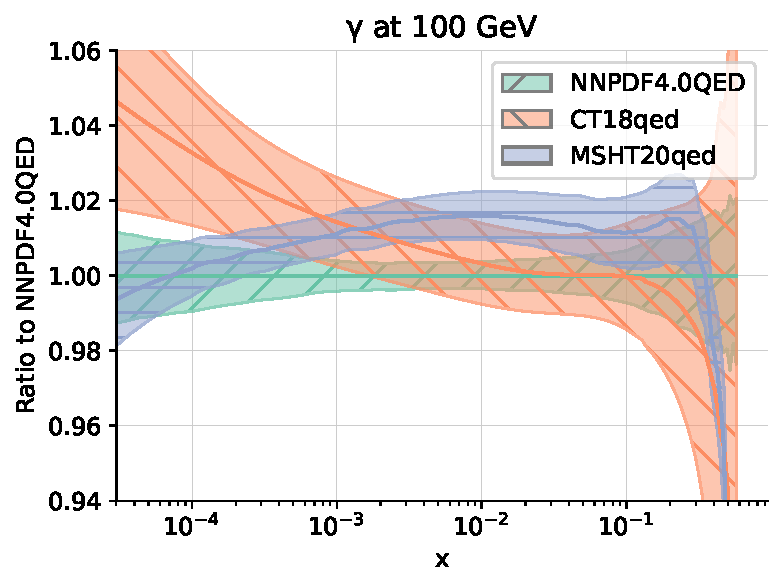
\includegraphics[width=0.3\textwidth]{figures/photon_comparison.pdf}
%     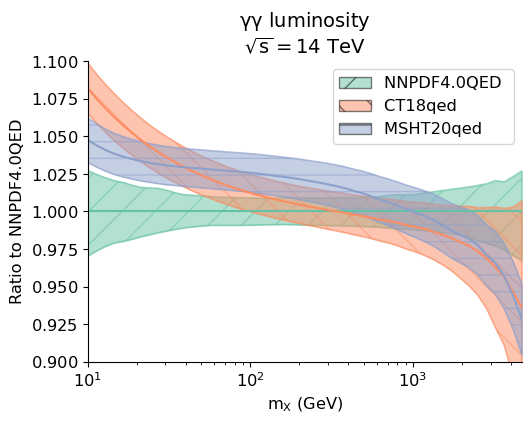
\includegraphics[width=0.3\textwidth]{figures/pp_lumi_comparison.png}
%     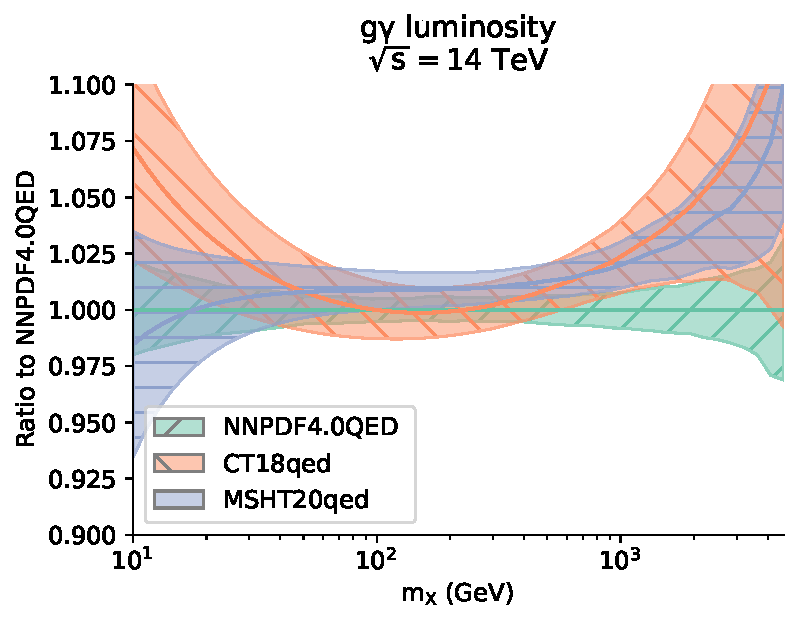
\includegraphics[width=0.3\textwidth]{figures/gp_lumi_comparison.pdf}
%   \end{center}
%   \begin{itemize}
%     \item Because all groups use the luxQED formalism, the photon PDFs agree at percent level
%     \item Luminosity generally in agreement, but differ at very small and very large invariant mass
%   \end{itemize}
% \end{frame}


% ============================================================================


\begin{frame}{Incomplete higher order uncertainties covmat}
  \begin{itemize}
    \item We construct an IHOU matrix following a similar approach by varying the subleading functions
    \item IHOU are independent of MHOU so the uncertainties are added in quadrature
    $$C = C_\mathrm{exp}+C_\mathrm{MHOU}+C_\mathrm{IHOU}$$
  \end{itemize}

  \begin{columns}
    \begin{column}{0.49\textwidth}
      \begin{figure}[!t]
        \centering
        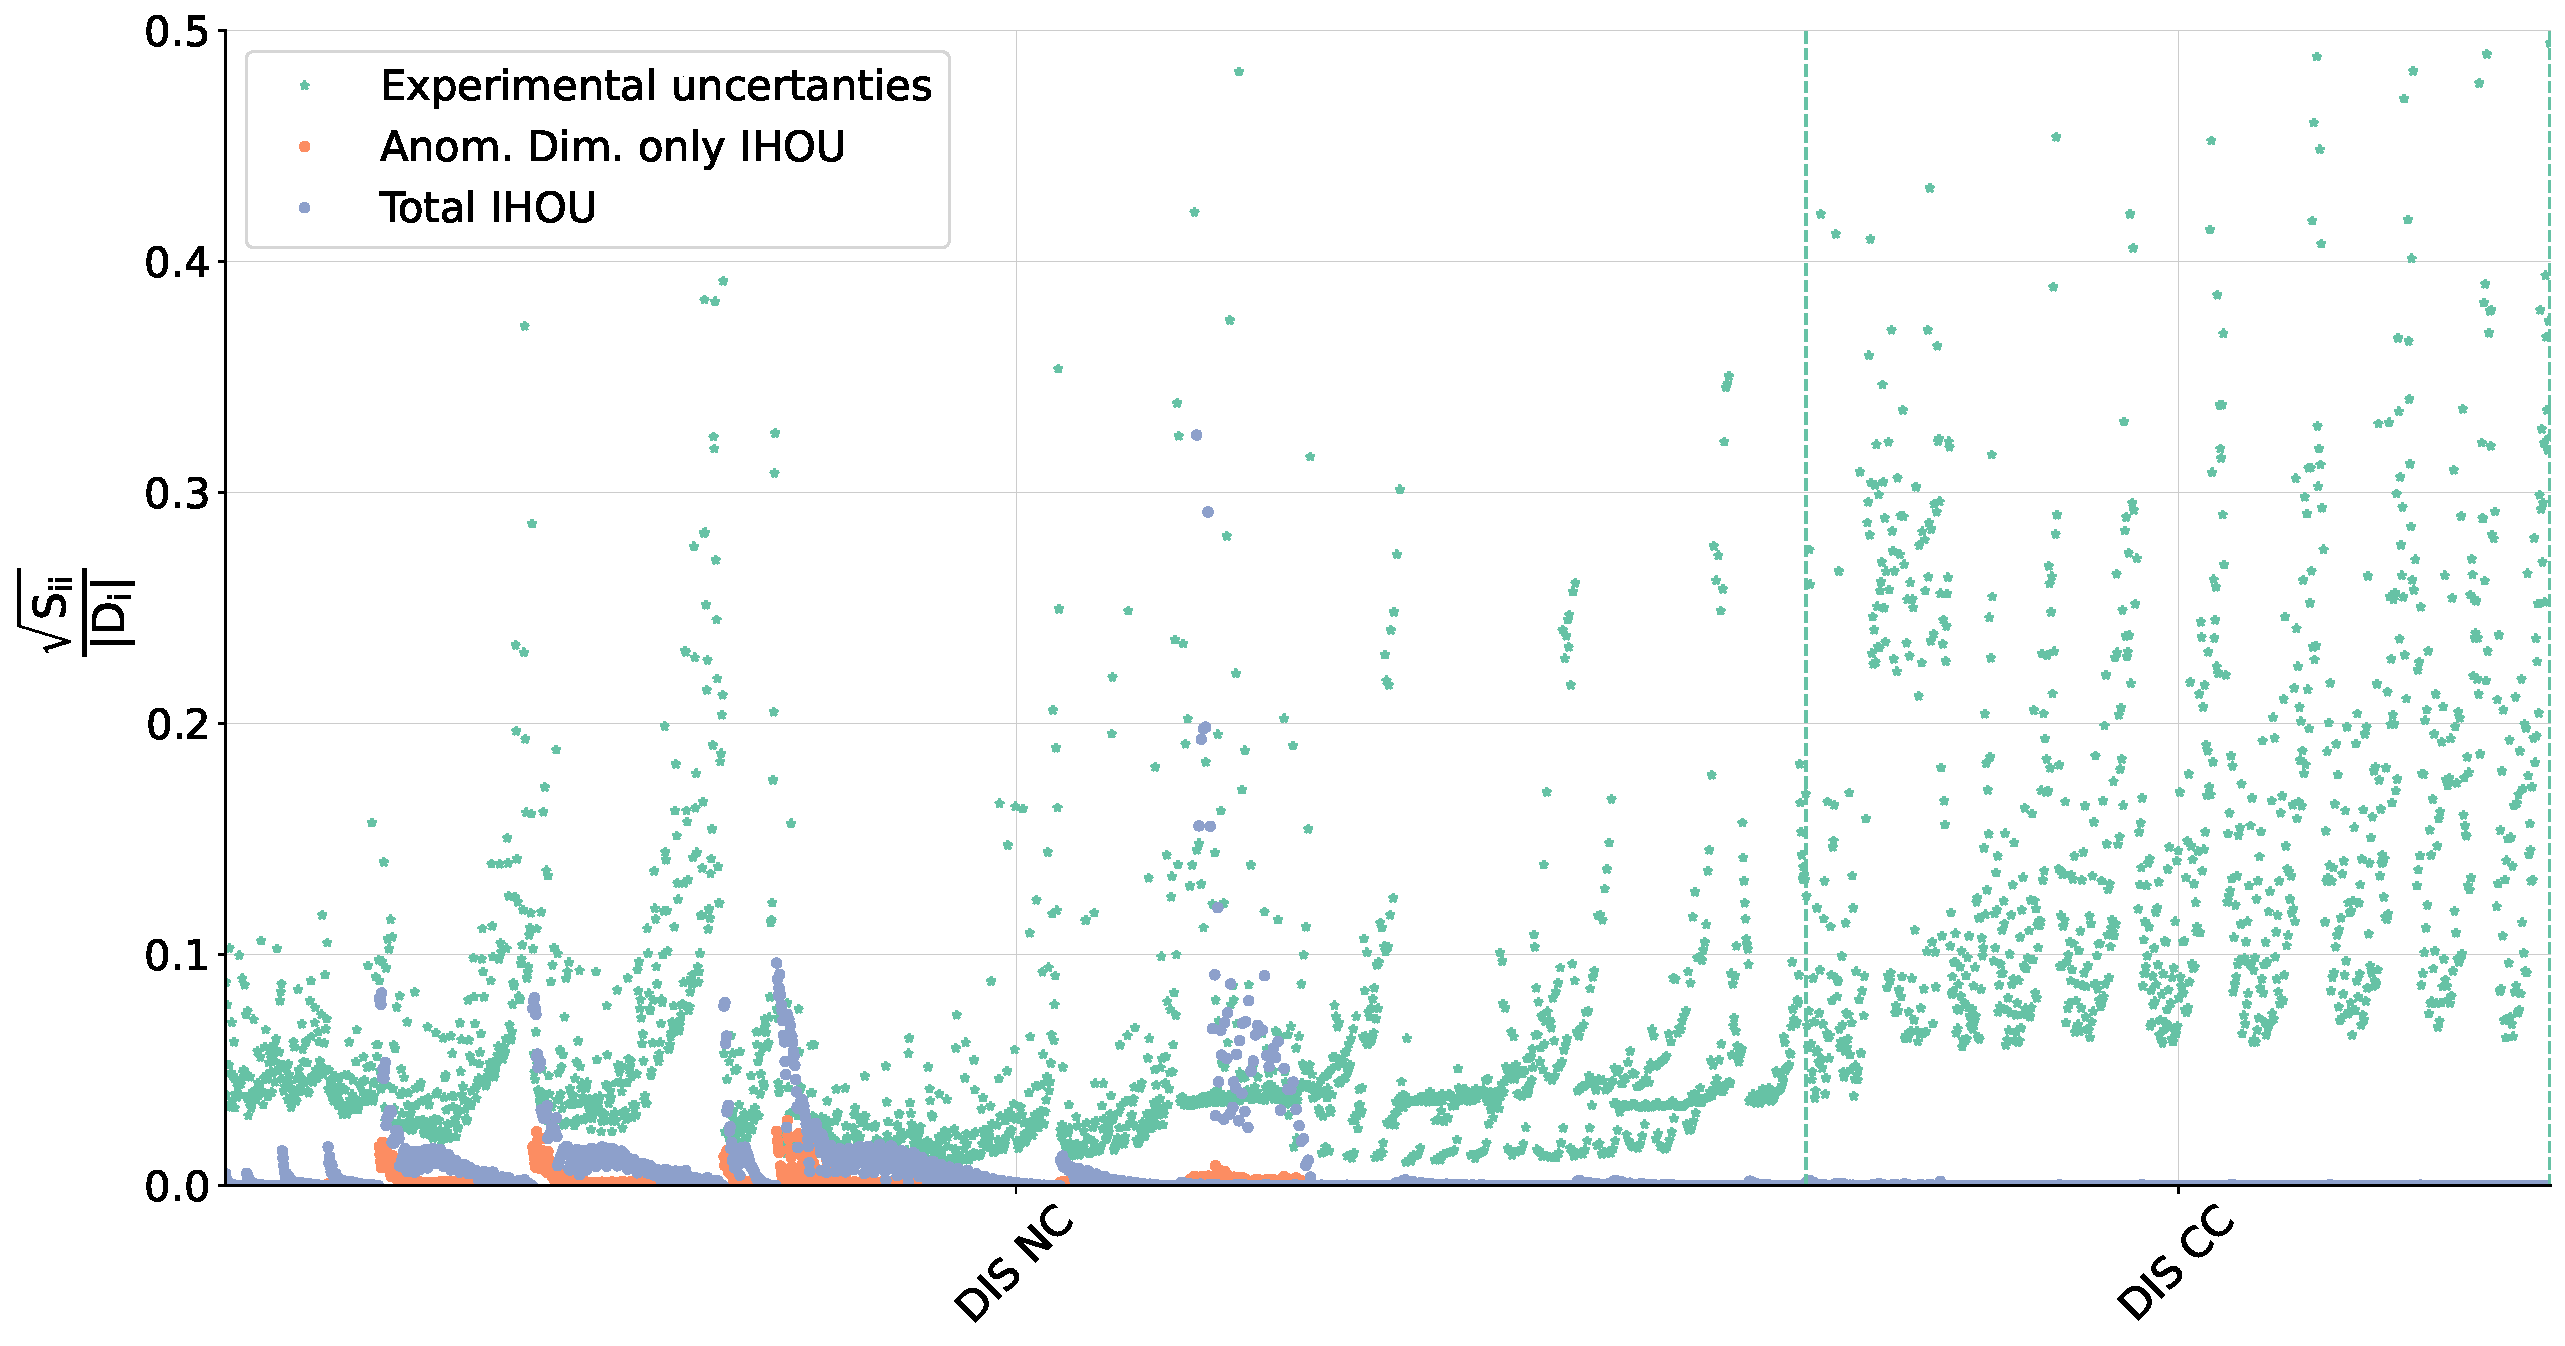
\includegraphics[width=.9\textwidth]{figures/diag_cov_dis_ihou.pdf}
        \caption*{IHOU have a large effect on small-$x$, low-$Q$ DIS data
        }
      \end{figure}
    \end{column}
    \begin{column}{0.49\textwidth}
      \begin{figure}[!t]
        \centering
        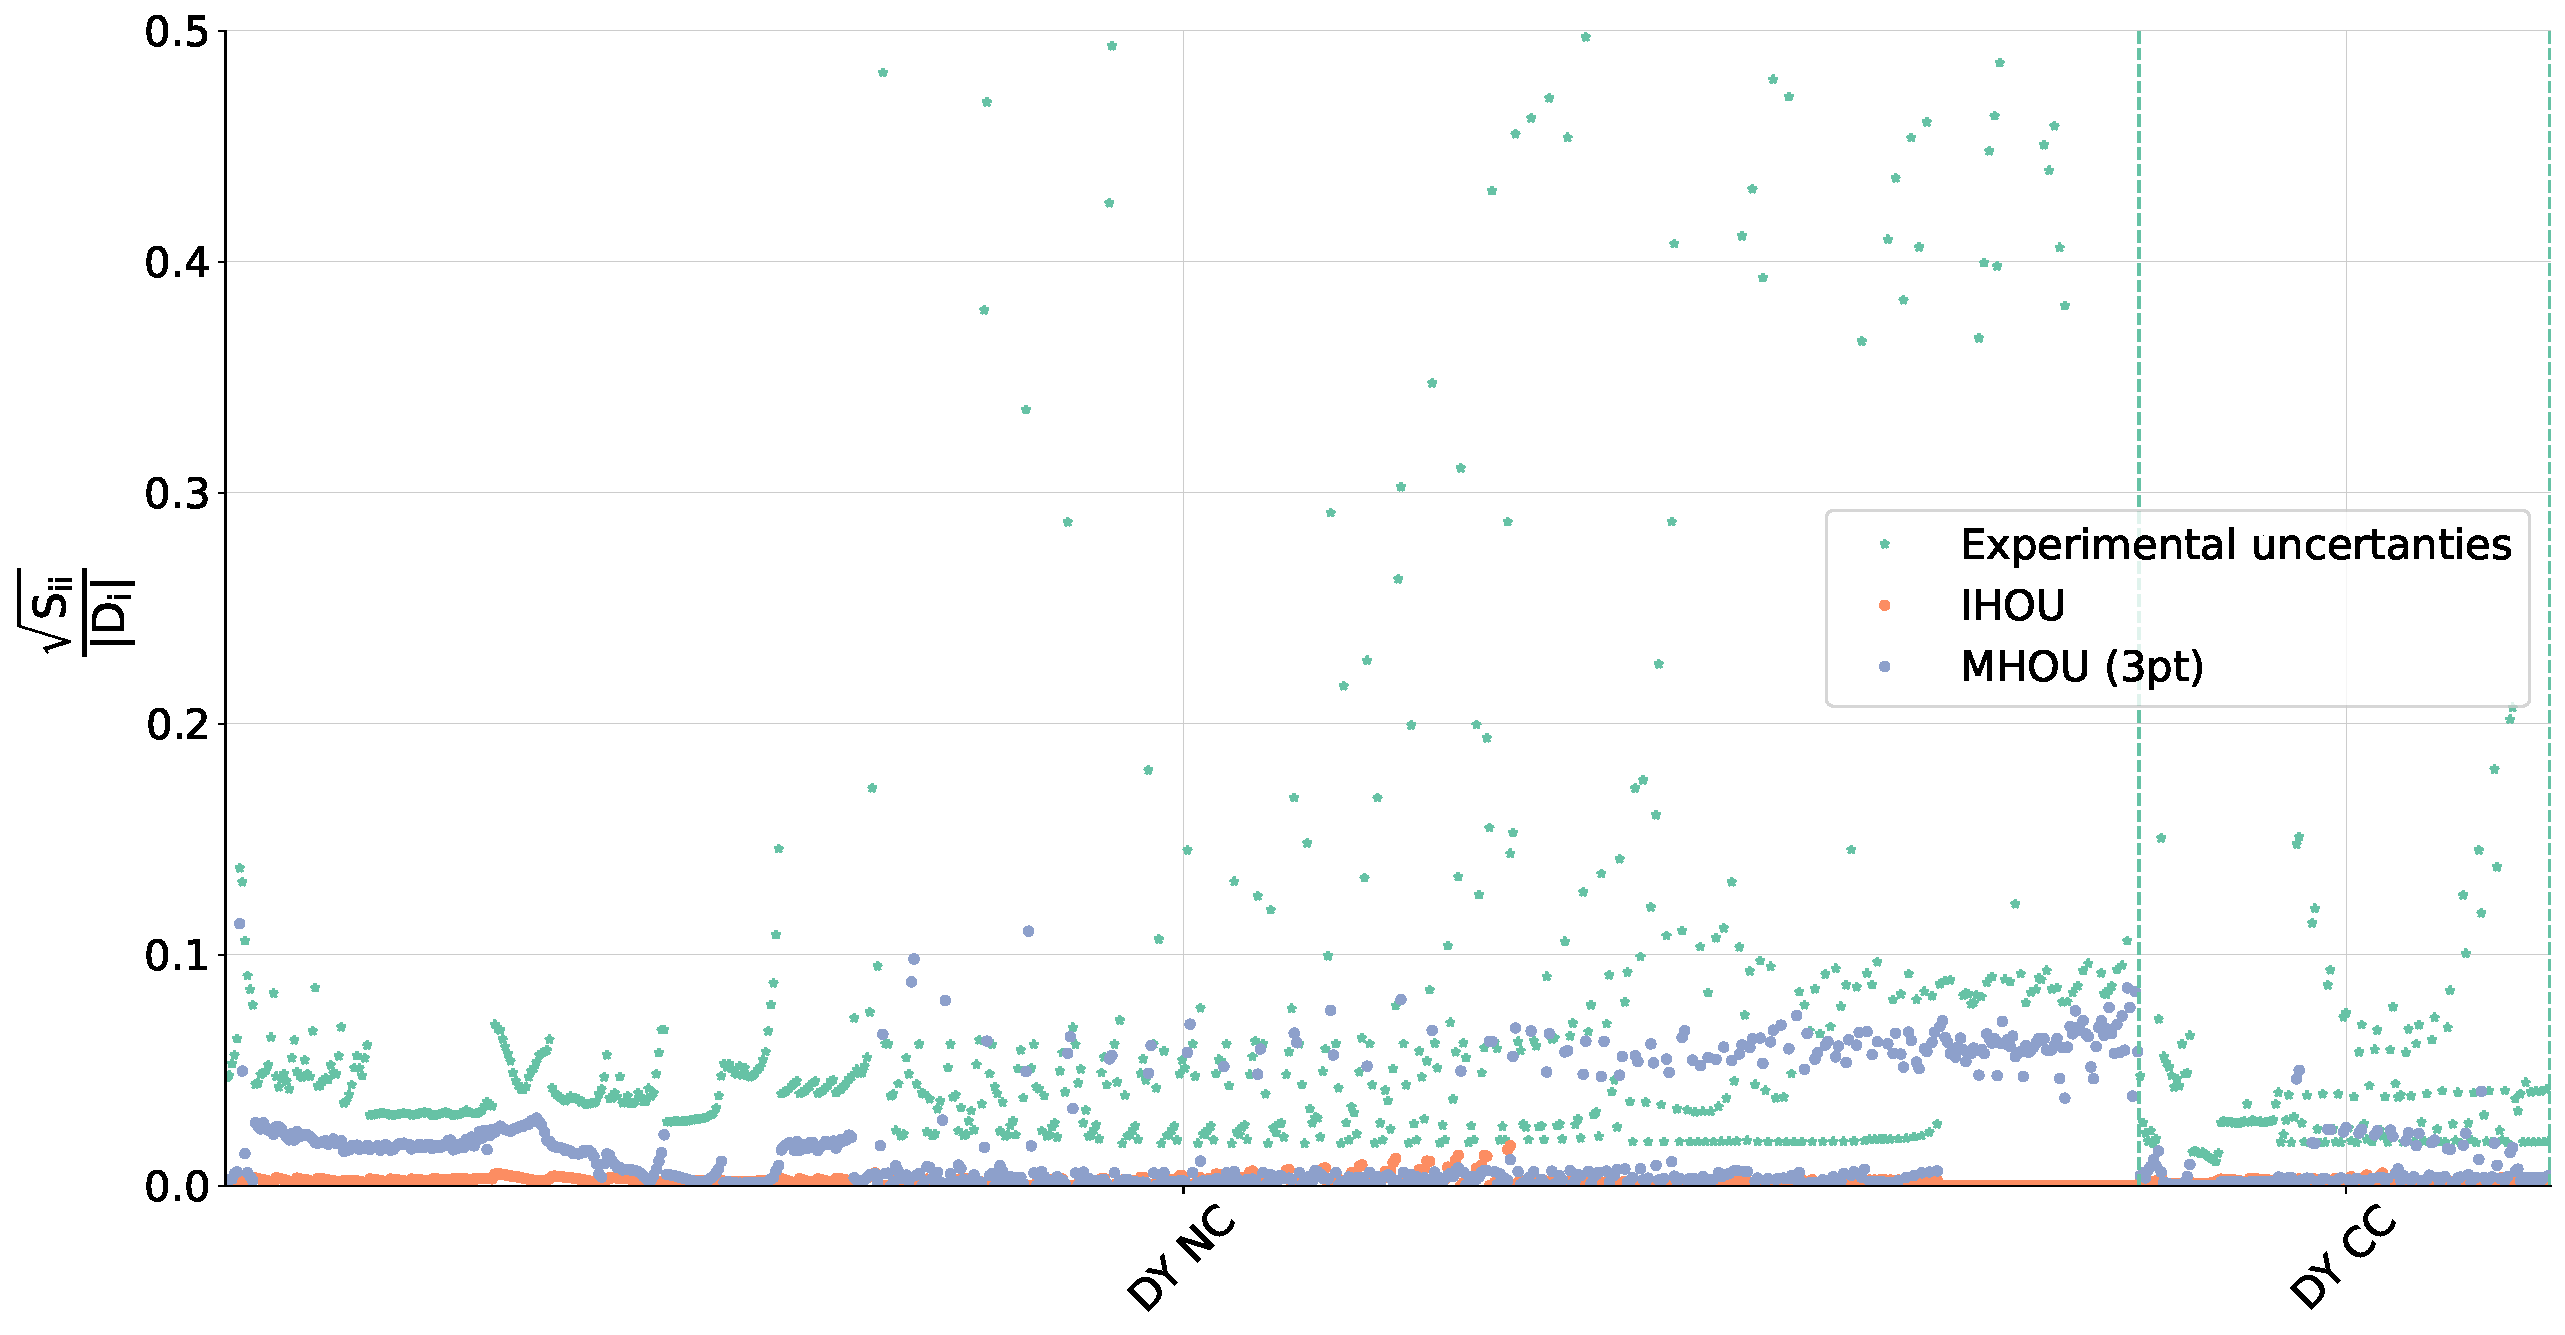
\includegraphics[width=.9\textwidth]{figures/diag_cov_dy_ihou_3pt_mhou.pdf}
        \caption*{NNLO MHOU included where N3LO not available \\
          MHOU can similar magnitude as the experimental uncertainty
        }
      \end{figure}
    \end{column}
  \end{columns}


\end{frame}

% \begin{frame}{Magnitude of theory uncertainties}
% % show that for certain processes th unc is of same size as exp unc.
% \end{frame}

% ============================================================================

\begin{frame}{Impact of MHOUs at N3LO}
  \begin{figure}[!t]
    \centering
    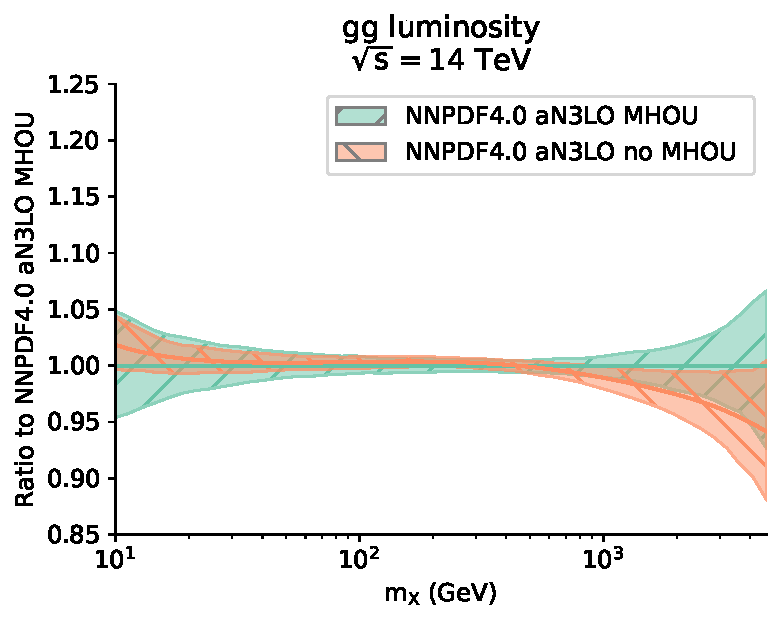
\includegraphics[width=0.45\textwidth]{figures/gg_plot_lumi1d.pdf}
    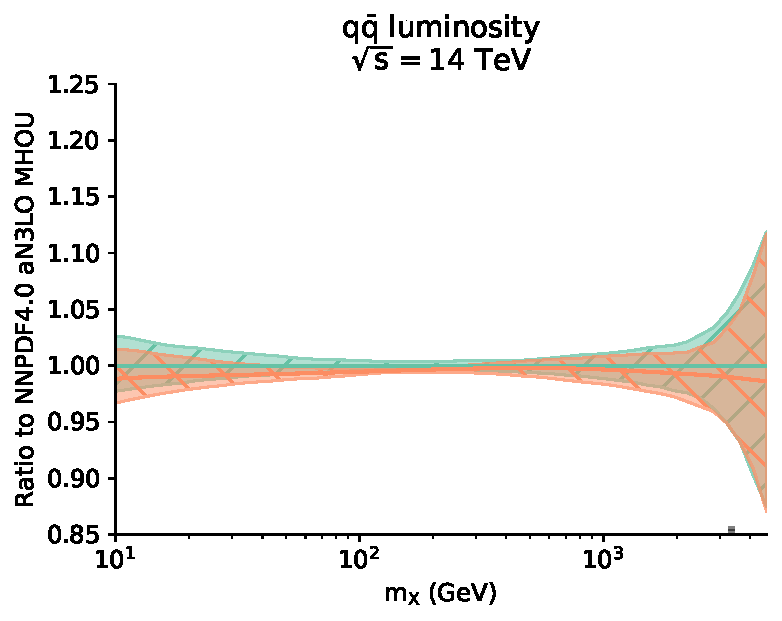
\includegraphics[width=0.45\textwidth]{figures/qqbar_plot_lumi1d.pdf}
  \end{figure}
  \begin{itemize}
    \item Non-negligible impact of MHOUs even at N3LO
    \item[$\Rightarrow$] reason to include exact N3LO calculations for hadronic processes
  \end{itemize}
\end{frame}


% \begin{frame}{Comparison to MSHT20}
%   \begin{figure}[!t]
%     \centering
%     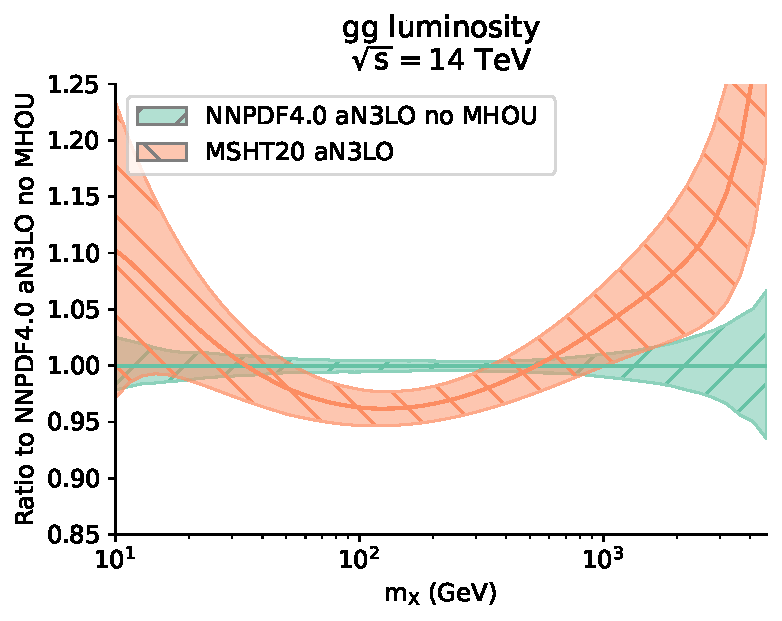
\includegraphics[width=0.45\textwidth]{figures/gg_plot_lumi1d_msht20.pdf}
%     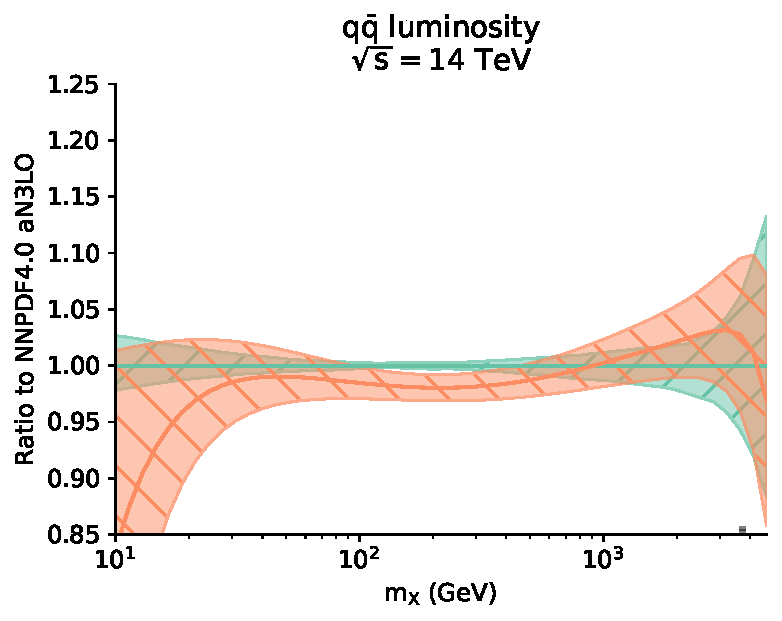
\includegraphics[width=0.45\textwidth]{figures/qqbar_plot_lumi1d_msht20.pdf}
%   \end{figure}
%   \begin{itemize}
%     \item Good agreement with MSHT20 for the quark luminosities
%     \item Also for gluon luminosities, except around the Higgs mass and high-mass
%     \item Similar data but different methodology (including splitting function parametrization)
%   \end{itemize}
% \end{frame}












\end{document}
